\documentclass[12pt,oneside, openany]{book}


\usepackage[paper = a4paper,
	bindingoffset = 2mm,     %Offset for binding side of page
	hmargin = 25mm,          %Left and right margin
	vmargin = 25mm,          %Top and bottom margin
	dvipdfm]
	{geometry}

\usepackage[utf8]{inputenc}

\usepackage[T1]{fontenc}	% Activate Type 1 fonts
\usepackage{mathptmx}       % Use Times font, also for math
\usepackage[scaled]{helvet} % for sans serif fonts (\textsf{...} or \sffamiliy)

\usepackage{fixltx2e} % Support subscript, superscript, etc.


\usepackage{graphicx}       % Handles figures
\usepackage{amsmath}
\usepackage{amsfonts}
\usepackage[mathcal]{euscript} % For calligraphy fonts
\usepackage{booktabs}       % Publication quality tables
\usepackage{setspace}       % Easy setting of line spacing

\usepackage{hyperref} % makes table of contents clickable

\usepackage{tocloft} % Required for modifying table of contents

\usepackage{listings}
\usepackage{xcolor}
\usepackage{caption}

% Custom JSON language definition
\lstdefinelanguage{json}{
    basicstyle=\normalfont\ttfamily,
    numbers=left,
    numberstyle=\tiny\color{gray},
    stepnumber=1,
    numbersep=8pt,
    showstringspaces=false,
    breaklines=true,
    frame=single,
    backgroundcolor=\color{white},
    literate=
        *{0}{{{\color{blue}0}}}{1}
         {1}{{{\color{blue}1}}}{1}
         {2}{{{\color{blue}2}}}{1}
         {3}{{{\color{blue}3}}}{1}
         {4}{{{\color{blue}4}}}{1}
         {5}{{{\color{blue}5}}}{1}
         {6}{{{\color{blue}6}}}{1}
         {7}{{{\color{blue}7}}}{1}
         {8}{{{\color{blue}8}}}{1}
         {9}{{{\color{blue}9}}}{1}
         {:}{{{\color{red}{:}}}}{1}
         {,}{{{\color{red}{,}}}}{1}
         {\{}{{{\color{red}{\{}}}}{1}
         {\}}{{{\color{red}{\}}}}}{1}
         {[}{{{\color{red}{[}}}}{1}
         {]}{{{\color{red}{]}}}}{1},
}

\lstset{
    basicstyle=\ttfamily,
    columns=fullflexible,
    breaklines=true,
    postbreak=\mbox{\textcolor{red}{$\hookrightarrow$}\space},
    frame=single,
    captionpos=b,
    numbers=left,
    numberstyle=\tiny\color{gray}
}

% Add dotted lines between chapter/section/subsection titles and page numbers
\renewcommand{\cftchapleader}{\cftdotfill{\cftdotsep}}
\renewcommand{\cftsecleader}{\cftdotfill{\cftdotsep}}
\renewcommand{\cftsubsecleader}{\cftdotfill{\cftdotsep}}

\hypersetup{hidelinks}

\hypersetup{
	colorlinks,      % Colored links
	colorlinks,      % Colored links
	citecolor=black,  % Color of cite links
	linkcolor=black,  % Color of links
	urlcolor=blue,   % Color of urls
}

\usepackage[style=numeric]{biblatex}
\usepackage{csquotes}


\addbibresource{refrences.bib}

\usepackage{titlesec}

% Variables
\newcommand{\thesisTitle}{Insights into Maritime Shipping's Carbon Footprint}
\newcommand{\thesisSubtitle}{Assessing the State of Emissions in Maritime Shipping Through Big Data Analysis}
\newcommand{\authorName}{Freddy Rameshchandra Thobhani}
\newcommand{\ProgramName}{Masters in Green Energy Technology (Smart Energy) }
\newcommand{\DepartmentName}{Department of Engineering}
\newcommand{\supervisorName}{Lucian Mihet-Popa}

\captionsetup{font=small, labelfont=it, textfont=it}


\begin{document}


\begin{titlepage}

    \begin{flushright}
        \includegraphics*[width=74mm]{images/logo.png}
    \end{flushright}

    \vspace{2cm}



    % Title
    \noindent{\LARGE\textbf{\thesisTitle}}

    \vspace{0.5cm}

    % Subtitle
    \noindent{\large {\thesisSubtitle}}

    \vspace{1cm}

    % Author Name
    \noindent{\large \authorName}


    \noindent\vspace{1cm}

    % program name
    \noindent{\large \ProgramName}

    \vspace{0.5cm}

    % department name
    \noindent{\large \DepartmentName}

    \vspace{1cm}

    % supervisor name
    \noindent{\large Supervisor: \supervisorName}

    \vspace{2cm}

    % Date
    \noindent{\large \today}

    \centering
    \vspace*{\fill}
    \includegraphics*[width=\textwidth]{images/cover.png}

    \thispagestyle{empty} % exclude from page numbering
\end{titlepage}

\begin{titlepage}
    \def \and {\\}
    \null\vfill
    \centering

    % Title
    {\fontsize{24}{28pt} \textbf{\thesisTitle}}

    \vfill


    % Subtitle
    {\fontsize{20}{23pt} \textit{\thesisSubtitle}}

    \vfill

    % Author Name
    {\fontsize{16}{18pt} \authorName}

    \vfill\vfill\vfill

    \thispagestyle{empty} % exclude from page numbering
\end{titlepage}


\chapter*{Preface}
\addcontentsline{toc}{chapter}{Preface}

This thesis marks final work of my 2 years long Master of Science degree within \ProgramName at \DepartmentName. 
The thesis is the result of a 6 month long research project, which I have conducted at Østfold under supervion of \supervisorName. 
The project has been conducted in collaboration with Astrup Fearnley, and has been supervised by Kristian Amundsen Ruud and corresponds to  30 ECTs.

\vspace{30pt}


\begin{center}
    Fredrikstad, \today
    \vspace{40pt}

    \authorName
\end{center}

\pagenumbering{roman} % Set page numbering to roman for the beginning

\chapter*{Abstract}
\addcontentsline{toc}{chapter}{Abstract}
\setlength{\parskip}{1em}

Maritime shipping stands as a pivotal pillar within the global economy, 
facilitating the transportation of over 90\% of the world's commodities and also major contributor to carbon emissions.
Maritime industy is a very volatile system  generating very large and complex data sets.
Employing the robust framework of Big Data analysis, this thesis explores the carbon emissions of maritime shipping through indicators like Carbon Intensity Indicator (CII) and Energy Efficiency Operating Indicator (EEOI).
Analysing emissions of about 9400 vessels grouped by segments and assigning them A to E grade based on their emissions helps us to understand complexity of emissions in maritime shipping with simple grading system.


The projection of Carbon Intensity Indicator (CII) trends for the period 2023 to 2026 elucidates a concerning pattern: a growing number of vessels may soon be graded D or E due to elevated carbon intensity.
The examination of the interplay between vessel speed, EEOI, and grade exposes noteworthy insights. It is evident that vessels exhibiting lower speed and reduced EEOI tend to achieve superior grades.
This revelation helps to inovate to find practical and cost-effective pathways for emissions mitigation, 
including measures such as the reduction of vessel speed, the implementation of low friction coatings, and the diligent maintenance of propellers and hulls.


This thesis makes significant strides in advancing our comprehension of maritime shipping's carbon impact. 
By offering pragmatic solutions, it not only addresses a pressing concern but also lays the groundwork for responsible and informed industry practices.
\chapter*{Acknowledgements}
\addcontentsline{toc}{chapter}{Acknowledgements}

I am deeply grateful to the numerous individuals who have played a crucial role in the successful completion of this thesis. 
First and foremost, I extend my sincerest appreciation to Professor Nicolae Lucian Mihet at Østfold University College, 
whose guidance, insights, and unwavering support have been invaluable throughout this research journey. 
I am also grateful to my supervisor, Kristian Amundsen Ruud, at Astrup Fearnley, for his expertise, thought-provoking ideas, and continuous support, which have significantly enriched the outcomes of this project.

I am equally thankful for the collaborative spirit and shared wisdom of the exceptionally talented team at Astrup Fearnley, with whom I had the privilege of working. 
Their support and contributions have undeniably elevated the quality of this work. 
I would like to express my sincere gratitude to my friends and family for the unwavering support and encouragement, who have been a constant source of motivation during this challenging academic pursuit.

While it is impossible to individually name all contributors, I wish to extend my heartfelt thanks to everyone who has contributed to this thesis in diverse ways. 
Your collective influence has been instrumental in shaping this endeavor, and your impact resonates profoundly in the culmination of this achievement.


\tableofcontents
\addtocontents{toc}{\protect\thispagestyle{empty}}

\newpage
\listoffigures

\listoftables



\pagenumbering{arabic} % Switch back to arabic numbering for the first chapter
\setlength{\parskip}{\baselineskip} % Set paragraph spacing to 1 line

\chapter{Introduction}
\setcounter{page}{1}

\section{Background and Motivation}

In the 21st century, Climate change is the biggest challenge faced by humanity. It poses a substantial danger to the survival of the inhabitants of our planet.
Human activities such as deforestation and burning of fossil fuels have led to a rise in global temperatures.
Becuase of this rise, there has been a rise in sea levels, extreme weather events, and loss of biodiversity.
There is an urgent need to reduce greenhouse gas emissions and transition to a sustainable, low-carbon future.

Maritime is essential to the global economy, transporting 90\% of the world's goods by volume.
It is also a major source of greenhouse gas emissions, with the International Maritime Organization (IMO)
estimating that maritime shipping accounts for 3\% of global carbon dioxide emissions.
While 3\% may seem small, it is important to note that this is a rapidly growing sector.
Without action, maritime shipping contribution to carbon emissions can increase upto 10-13\% in the next few decades..
Due to this fact, there is a growing global effort to reduce emissions from this sector. \autocite{king_anthony_2022}.

In accordance with sustainable Development Goal 13, in 2018, the inital stratergy was adopted by IMO's Environmental Protection Committee (MEPC),
during its 72nd session at IMO Headquarters in London, United Kingdom. Accorging to this stratergy,
the IMO will work towards reducing the total annual greenhouse gas emissions from international shipping by at least 50\% by 2050 compared to 2008 \autocite{imo-2018}.
In 76th ssssion MEPC in 2021, serval mandatory measures were adopted to reduce greenhouse gas emissions from international shipping,
which will help in achieving the goal of reducing emissions by 50\% by 2050 \autocite{imo-2021}. One of the important measures is the carbon intensity indicator (CII).

\begin{figure}[ht]
    \centering
    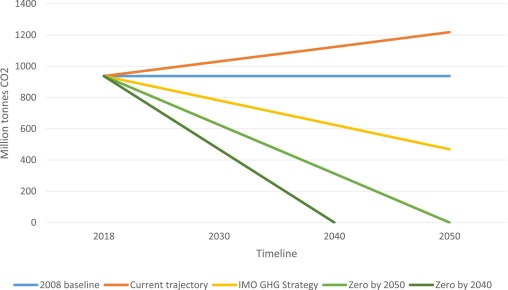
\includegraphics[width=0.7\textwidth]{images/emission_trajactory.jpg}
    \caption{Emission trajectories for different levels of ambition for emission reduction targets}
    \label{emissionTrajectory}
\end{figure}


Maritime shipping is a complex and highly volatile system, generating very large data sets.
Big data analytics can be used to understand the complex system and make informed decisions.
It can facilitate operations such as monitoring of emission and predictive analysis of vessel performance.
This can help in reducing emissions and improving the efficiency of the maritime sector \autocite{ZAMAN2017537}.


\section{Big Data Analysis}

Big data analytics is where advanced analytic techniques operate on big data sets. Hence, big data
analytics is really about two things — \textit{big data} and \textit{analytics}.



\subsection{Big Data}

As the name suggests, big data is a large amount of data. There are other important attributes of big data. These are:  data variety and data velocity.

Thus we can define big data using 3 V's: \textit{volume}, \textit{variety}, and \textit{velocity} as showin in figure \ref*{bigData}.

\begin{figure}[h]
    \centering
    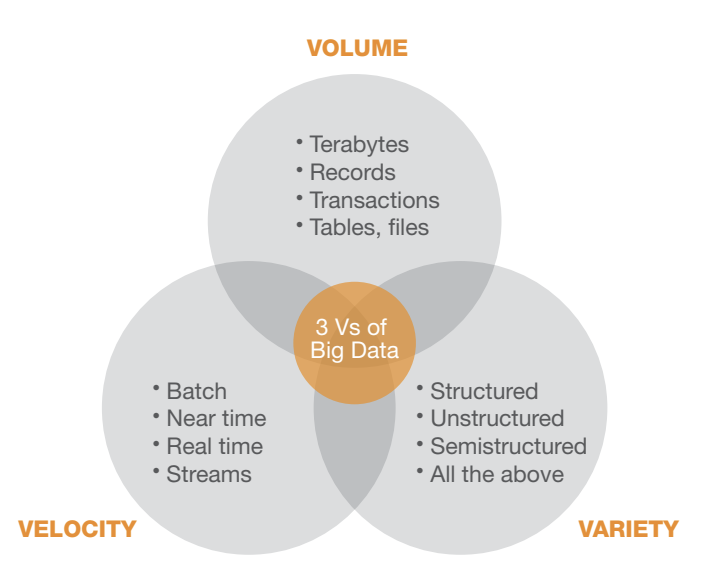
\includegraphics[width=0.5\textwidth]{images/big_data.png}
    \caption{Big Data: 3 V's \autocite{3vbigdata}}
    \label{bigData}
\end{figure}

Beyond these three V's, Big Data is also about how complicated the computing
problem is. Given the number of variables and number of data points for analysing the maritime shipping data. It is a very complicated problem.
Thus, in addition to the three V's identified by IBM, it would also be necessary to take complexity into account as shown in figure \ref*{bigDataComplex} \autocite{pence2014big}.

\begin{figure}[h]
    \centering
    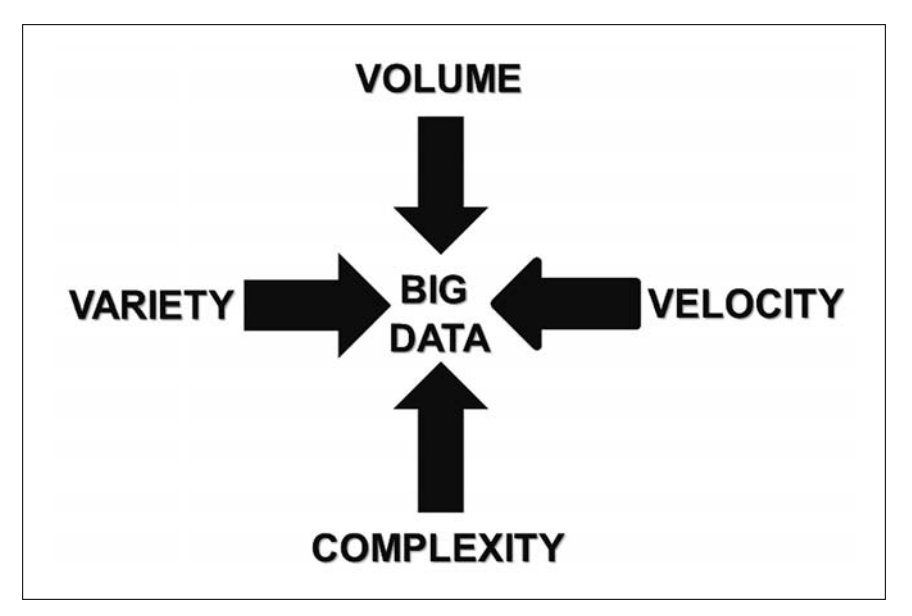
\includegraphics[width=0.5\textwidth]{images/big_data_complex.png}
    \caption{Big Data: Beyong 3 V's - volume, velocity,
        variety, and complexity}
    \label{bigDataComplex}
\end{figure}


\subsection{What is Big Data Analytics?}

Big data analytics is the process of examining large and varied data sets to uncover hidden patterns, unknown correlations, market trends, customer preferences and other useful information that can help organizations make more-informed business decisions.

Thus, Data analytics revolves around deriving valuable knowledge and meaningful insights from extensive sets of data.
This process involves crafting hypotheses, often rooted in gathered experiences and uncovering correlations between variables, sometimes even through serendipitous discoveries.
Data analytics can be classified into four distinct types \autocite{rajaraman2016big}:

\subsubsection{1. Descriptive Analytics}

Descriptive analytics focuses on explaining past events and presenting them in a comprehensible manner.
The collected data is structured into visual aids like bar charts, graphs, pie charts, maps, and scatter diagrams, facilitating easy interpretation that offers insights into the data's implications.
This mode of data representation is often termed a dashboard, reminiscent of a car's dashboard that provides details such as speed, engine status, fuel levels, and distance traveled.
A classic instance of descriptive analytics involves displaying population census data, which categorizes a nation's population by gender, age brackets, education, income, population density, and similar criteria \autocite{rajaraman2016big}.

\subsubsection{2. Predictive Analytics}

Predictive analytics extends beyond existing data to forecast forthcoming events.
It anticipates what is likely to occur in the immediate future.
Techniques like time series analysis utilizing statistical methods, neural networks, and machine learning algorithms are employed for this extrapolation.
A significant application of predictive analytics is seen in marketing, where it understands customer preferences and needs.
For instance, when purchasing shoes online, an advertisement for socks may appear.
Another prevalent application is in orchestrating election campaigns.
This involves gathering diverse data, such as the demographics of voters in different areas and their perceived needs like infrastructure and local concerns \autocite{rajaraman2016big}.

\subsubsection{3. Prescriptive Analytics}

This process detects opportunities for enhancing existing solutions by analyzing collected data.
Essentially, it guides us on the actions to undertake in order to accomplish a particular objective.
An illustrative instance is observed in the aviation industry where airlines determine seat pricing through analysis of historical travel patterns, popular travel origins and destinations, significant events, holidays, and more.
This approach is employed to optimize profit generation \autocite{rajaraman2016big}.

\subsubsection{4. Exploratory or Discovery Analytics}

This process uncovers unforeseen connections among variables within extensive datasets.
The collection and analysis of data from diverse sources opens up new avenues for gaining insights and making serendipitous discoveries.
One of its major applications involves the identification of patterns in customers' behavior by companies through sources like feedback, tweets, blogs, Facebook data, emails, and sales trends.
By deciphering customer behavior, companies can potentially predict actions like renewing a magazine subscription, switching mobile phone service providers, or canceling a hotel reservation. Armed with this information, companies can devise appealing offers aimed at altering the anticipated course of action by the customer \autocite{rajaraman2016big}.
\section{Problem Statement}

Carbon emissions from maritime shipping have been identified as a major contributor to global greenhouse gas emissions, with the International Maritime Organization estimating that shipping is responsible for around 3\% of global CO2 emissions \autocite{king_anthony_2022}.
To address this issue, the shipping industry has set targets to reduce its carbon footprint, and governments and international organizations have introduced policies and regulations to encourage emissions reduction.

However, measuring and monitoring carbon emissions from maritime shipping can be challenging due to the complexity of the industry and the lack of reliable data.
The Energy Efficiency Existing Ship Index (EEXI) and the Carbon Intensity Indicator (CII) have been proposed as two metrics to assess the carbon efficiency of ships and enable comparison between different vessels and fleets \autocite{ZHANG2019118223,CHUAH2023115348}.
However, there is a need to better understand the relationship between EEXI and carbon emissions, as well as to identify the factors that influence EEXI.

Therefore, the aim of this thesis is to conduct a big data analysis of carbon emissions in maritime shipping, using EEXI as the main metric. Specifically, the study will:

\begin{itemize}
    \item Calculate EEXI for a sample of vessels using real-world data on fuel consumption and other operational parameters.
    \item Analyze the relationship between EEOI, CII, and carbon emissions, using statistical methods and machine learning algorithms.
    \item Identify the factors that influence EEXI and CII, such as vessel age, size, speed, and route, and examine their impact on carbon emissions.
    \item Evaluate the usefulness of EEXI and CII as metrics for monitoring and reducing carbon emissions in maritime shipping, and recommend potential improvements to these metrics.
\end{itemize}


Overall, the findings of this thesis will contribute to a better understanding of the carbon efficiency of maritime shipping and inform the development of policies and strategies for emissions reduction in this sector.
\section{Research Question}

This theis will focus on answering following research questions:

\begin{enumerate}
    \item What is the relationship between vessel age and carbon emissions in maritime shipping?
    \item How do shipping routes affect carbon emissions in maritime shipping?
    \item What role do fuel types and engine technologies play in carbon emissions in maritime shipping?
    \item How can EEOI and CII be used to monitor and reduce carbon emissions in maritime shipping?
\end{enumerate}
\section{Report Outline}

\begin{figure}[ht]
    \centering
    \includegraphics[width=1\textwidth]{images/thesis_outline.png}
    \caption{Outline of the thesis}
    \label{fig:outline}
\end{figure}

\noindent Chapter 2: Litrature Review: This chapter covers the background information and literature review of the thesis.
this section covers comprehensive review of existing papers and research related to carbon emissions in maritime shipping.
The aim is to provide a comprehensive overview of the current state of research in this field and identify any gaps or opportunities for further exploration.


\noindent Chapter 3: Data Collection and Understanding:
In this chapter, the focus will be on gathering and understanding the data required to perform analysis to understand emissions in martime shipping.
Various data sources will be explored, including industry databases, research publications, and government reports.
The aim is to acquire a comprehensive dataset that covers different aspects of carbon emissions in the maritime sector.
Additionally, this chapter will delve into the intricacies of the collected data, understanding its structure, variables, and potential limitations.

\noindent Chapter 4: Data Cleaning and Preprocessing:
Before conducting any data analysis, it is crucial to ensure the quality and integrity of the dataset.
This chapter will discuss the steps involved in cleaning and preprocessing the data.
This process may involve handling missing values, dealing with outliers, standardizing formats, and resolving inconsistencies.
By performing these necessary data cleaning procedures, the dataset will be prepared for further analysis, ensuring reliable and accurate results.

\noindent Chapter 5: Data Analysis Techniques:
In this chapter, various data analysis techniques specific to big data will be explored and applied to the cleaned dataset.
These techniques may include statistical analysis, machine learning algorithms, and data visualization methods.
The goal is to extract meaningful insights and patterns from the data to gain a comprehensive understanding of carbon emissions in maritime shipping.
Additionally, this chapter will discuss the tools and technologies utilized for data analysis and highlight any specific challenges encountered during the process.

\noindent Chapter 6: Evaluation of Results:
After performing the data analysis, this chapter will focus on evaluating and interpreting the obtained results.
The findings will be compared against existing literature, industry benchmarks, and regulatory standards to assess the significance and implications of the analysis.
The strengths and limitations of the analysis approach will be discussed, and recommendations for future research or practical applications will be provided.
This chapter aims to provide a comprehensive evaluation of the insights gained from the data analysis and their potential impact on the maritime shipping industry.

\noindent Conclusion:
The conclusion chapter will summarize the key findings and contributions of the thesis.
It will highlight the significance of the conducted big data analysis on emissions in maritime shipping and its implications for sustainability and environmental initiatives.
The conclusion will also discuss any potential limitations or challenges encountered during the research and suggest avenues for further exploration in this field.
\chapter{Literature Review}

In response to the urgent need to reduce carbon emissions and combat climate change, researchers and industry stakeholders have focused on developing and implementing strategies to reduce carbon emissions in maritime shipping.

Figure \ref{publicationRate} shows that the number of publications on energy efficiency and emission reduction in the maritime industry has grown exponentially since 2016. The number of publications from 2006 to 2015 was 76, while from 2016 to 2021, there were 260 publications, indicating a significant increase in interest in decarbonization in the maritime industry.
\autocite{JIMENEZ2022132888}

\begin{figure}[h]
    \centering
    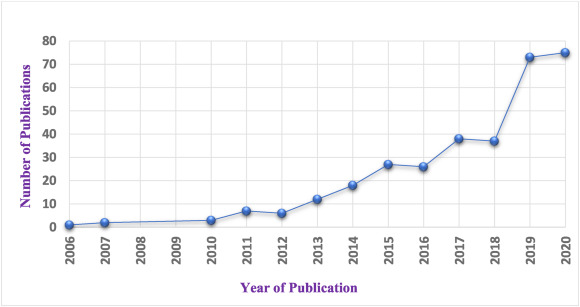
\includegraphics[width=0.7\textwidth]{images/publication_rate.jpg}
    \caption{Number of publications per year in energy efficiency and emission reduction in the maritime domain}
    \label{publicationRate}
\end{figure}

One promising area of research is the use of big data analysis to measure and improve carbon efficiency in maritime shipping. Big data analysis involves the collection and analysis of large and complex data sets to identify patterns, trends, and insights. In the context of maritime shipping, big data analysis can be used to measure carbon emissions and identify opportunities for improvement.

The purpose of this literatsure review is to examine the current state of research on carbon emissions in maritime shipping, with a focus on the Energy The Energy Efficiency eXisting ship Index (EEXI) and Carbon Intensity Indicator (CII) as key metrics for measuring carbon efficiency. The review will provide an overview of the current state of research on these metrics, their strengths and limitations, and their relevance for the maritime shipping industry.

The review will begin by exploring the importance of reducing carbon emissions in maritime shipping and the regulatory and policy frameworks that have been established to address this issue. It will then provide an overview of the EEXI and CII metrics, including their definitions, methodologies for calculating them, and their role in measuring carbon efficiency.

The literature review will also examine the current research on the relationship between EEXI, CII, and carbon emissions in maritime shipping, with a particular focus on the use of big data analysis to measure and improve carbon efficiency. It will explore the potential for big data analysis to provide more accurate and comprehensive data on carbon emissions, and to identify opportunities for operational and technological improvements.

Overall, this literature review will provide a comprehensive overview of the current state of research on carbon emissions in maritime shipping, with a focus on the EEXI and CII metrics and the potential for big data analysis to guide and inform strategies for improving carbon efficiency in the industry.


\section{Litrature Review}


Review by \citeauthor{en15217910} \autocite{en15217910} shows that Maritime shipping is a crucial aspect of global trade and the global economy, with over 85\% of the volume of global trade in goods transported by sea.
However, maritime transport also has significant environmental impacts, including carbon emissions.
Approximately 3.3\% of the world's carbon dioxide (CO2) emissions are attributable to maritime transport, with emissions from marine diesel oil (MDO), marine fuel oil (MFO), and heavy fuel oil (HFO) all contributing to the problem.
Reducing carbon emissions in the maritime shipping industry is a significant challenge, but there are a range of strategies that can be used to achieve this goal.
Alternative fuels, energy efficiency improvements, and operational measures all have the potential to reduce emissions, but they also have significant economic and resource constraints.


Paper by \citeauthor{en15176150} \autocite{en15176150} mentions that  Despite its significant contribution to global economic growth, maritime transport also generates negative externalities, primarily in the form of greenhouse gas (GHG) emissions.
They discus how digitalization and the use of artificial intelligence (AI) are being explored as potential ways to reduce emissions in maritime shipping.
AI algorithms can optimize shipping routes, reduce fuel consumption, and minimize emissions. Additionally, digitalization can enable better data collection and analysis, which can facilitate more accurate emissions reporting and monitoring.

According to \citeauthor{jmse10020129} \autocite{jmse10020129}, the use of automatic identification system (AIS) to estimate ship emissions, which is an advantage due to the system's ability to provide real-time navigational information.
Studies have been conducted utilizing AIS data to estimate ship emissions in different regions, such as Hong Kong and the Pearl River Delta, Las Palmas Port, Qingdao Port, Tianjin port, Naples port, and unidentified vessels with missing ship parameters.
The studies have focused on macro-scale spatial and temporal resolution, high-resolution ship emission inventory, high temporal-spatial ship emission inventory, higher spatial-temporal resolution, and real-time ship emission monitoring.
It proposes simulation model based on AIS data, specification and what-if scenarios as shown in Figure \ref{simaulationFramework}

\begin{figure}[h]
    \centering
    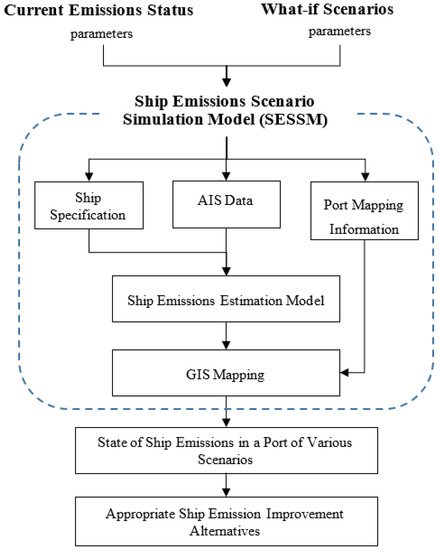
\includegraphics[width=0.5\textwidth]{images/simulation_framework.jpeg}
    \caption{Simulation framework}
    \label{simaulationFramework}
\end{figure}


Research by \citeauthor{SOU2022113239} \autocite{SOU2022113239}, discusses the need for carbon intensity indicators (CIIs) as performance monitoring tools in the shipping industry, particularly for tracking energy efficiency trends and progress towards climate targets.
The review highlights the lack of consensus on suitable CIIs, as proposed by various countries to the International Maritime Organization (IMO), and the need for a more comprehensive understanding of global progress towards carbon intensity targets from both demand and supply side indicators.
The study aims to address this issue by analyzing CIIs for shipping and the factors that influence the carbon intensity of shipping at the global level. Index decomposition analysis (IDA) is used to quantify the contribution of various factors, including energy efficiency, to changes in carbon intensity from 2012 to 2018.



According to report by \citeauthor{stevenson_2021_bulker} \autocite{stevenson_2021_bulker}, The International Maritime Organization will introduce Energy Efficiency eXisting ship Index (EEXI) and Carbon Intensity Indicator (CII) regulations in 2023 as part of the wider decarbonisation goals for shipping. More than three-quarters of the existing fleet will not initially meet EEXI baselines and will need to take action to achieve compliance, with overridable engine power limitations (oEPL) expected to be a popular option. However, the effect on vessel operations over a year will be quite small due to the relatively small number of hours where steaming speeds would exceed oEPL limits. The compliance with EEXI can result in modest improvements in AER, CII, and annual CO\textsubscript{2}. emissions.

\begin{figure}[h]
    \centering
    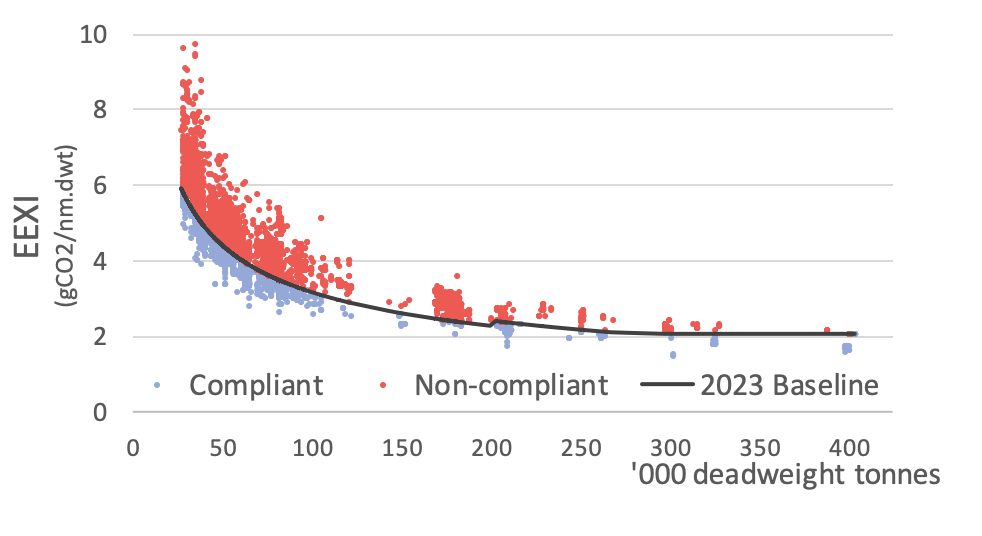
\includegraphics[width=0.7\textwidth]{images/eexi_non_compliant.png}
    \caption{EEXI BULKER ESTIMATES VS. 2023 BASELINE}
    \label{eexiNonCompliant}
\end{figure}


The International Maritime Organization (IMO) has made maritime decarbonization a priority, setting targets to reduce greenhouse gas emissions from ships.
To achieve these targets, the IMO has adopted mandatory measures, including the carbon intensity indicator (CII), which measures carbon emissions per unit transport work for each ship.
But \citeauthor{WANG2021100005} \autocite{WANG2021100005} argues there are potential paradoxes with the CII, as it may increase carbon emissions in some situations.
There are at least four potential versions of the CII, including supply-based, demand-based, distance-based, and sailing time-based, but the IMO has not yet agreed on which to use.
More elaborate models and indicators should be developed to analyze the potential impacts of the CII and achieve utmost carbon emissions reduction.

In \citetitle{doi:10.1080/03088839.2020.1788731} \autocite{doi:10.1080/03088839.2020.1788731}, author \citeauthor{doi:10.1080/03088839.2020.1788731} explains how Big data and artificial intelligence (AI) have become essential components of data-driven decision-making in most industries.
However, the maritime industry still relies on intuition more than on data, mainly because of the vast size of its network and planning problems.
The maritime industry generates large amounts of data that, if appropriately utilised in decision-making, can improve maritime safety, reduce environmental impacts, and minimise cost. In this review, we focus on studies that deal with big data and AI applications within the maritime context to map the conceptual structure of the field and identify future research avenues.
AIS data to investigate the impact of speed reduction on fuel consumption and carbon emissions in the shipping industry.
The study found that a 10\% reduction in ship speed could result in a 17\% reduction in fuel consumption and a corresponding reduction in carbon emissions.
The authors suggested that reducing ship speed is an effective way to reduce fuel consumption and carbon emissions in the maritime industry.

\begin{figure}[h]
    \centering
    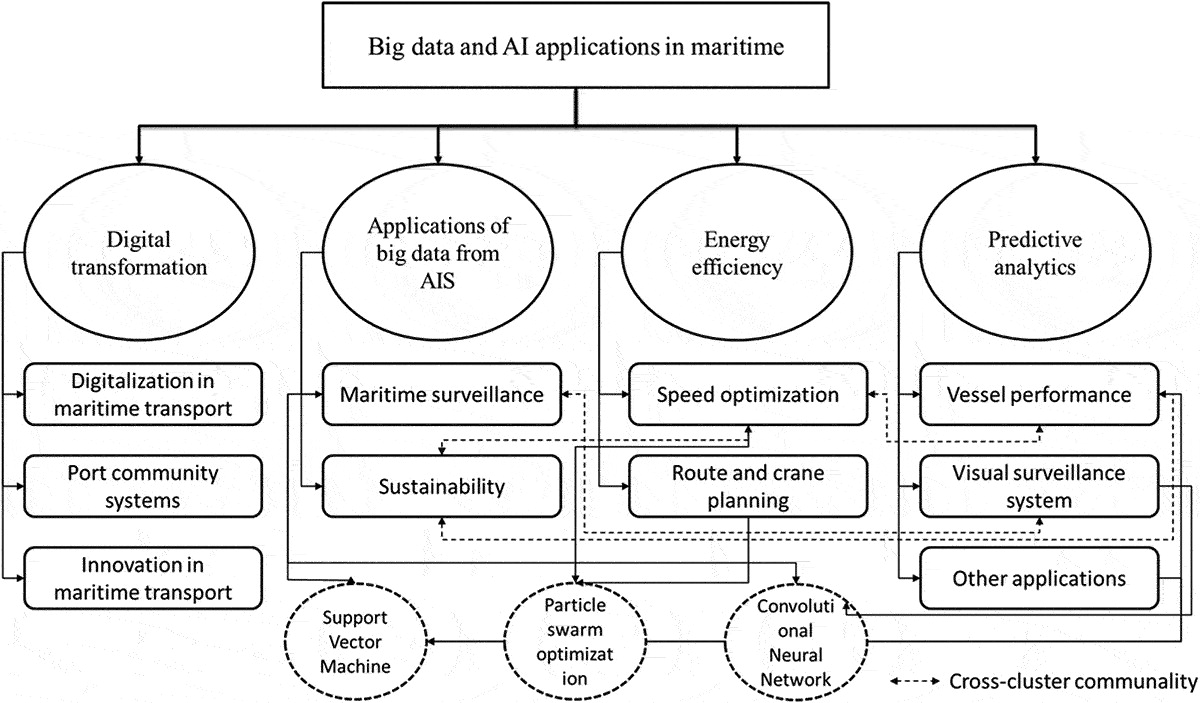
\includegraphics[width=0.7\textwidth]{images/application_big_data_martime.jpeg}
    \caption{Application of Big dada and AI in maritime industry}
    \label{applicationBigDataMartime}
\end{figure}

The study by \citeauthor{acomi2014improving} \autocite{acomi2014improving}, delves into the realm of maritime environmental conservation, emphasizing the Energy Efficiency Operational Index (EEOI) as a pivotal tool.
Addressing concerns of marine pollution encompassing water and air aspects, the paper underscores international efforts for emission reduction in shipping.
The EEOI, designed to measure carbon emissions per unit of transport work, aids ship-owners and operators in enhancing energy efficiency during operational voyages.
The research demonstrates how commercial software and a custom-developed program estimate EEOI values pre-voyage and onboard, revealing the influence of unpredictable factors on energy efficiency.
This analysis not only showcases the EEOI's significance in curbing emissions but also highlights its vital role in the broader context of maritime sustainability and environmental protection.

\subsection{Conclusion}

In this section, we have reviewed the literature on carbon emissions in maritime shipping, with a focus on the EEOI and CII metrics and the potential for big data analysis to guide and inform strategies for improving carbon efficiency in the industry.

In conclusion, the literature reviewed emphasizes the importance of addressing the significant environmental impact of carbon emissions in the maritime shipping industry.
While there are various strategies to reduce emissions, such as alternative fuels, energy efficiency improvements, and operational measures, they have significant economic and resource constraints.
Digitalization and the use of artificial intelligence (AI) are being explored as potential ways to reduce emissions by optimizing shipping routes, reducing fuel consumption, and minimizing emissions.
Furthermore, the use of automatic identification system (AIS) data can facilitate real-time emissions monitoring, while carbon intensity indicators (CIIs) can be used as performance monitoring tools.
The International Maritime Organization (IMO) has made maritime decarbonization a priority by setting targets to reduce greenhouse gas emissions from ships and introducing regulations like EEXI and CII.
However, potential paradoxes with the CII and lack of consensus on suitable CIIs highlight the need for more elaborate models and indicators to achieve utmost carbon emissions reduction. Big data and AI applications have the potential to improve maritime safety, reduce environmental impacts, and minimize costs.
Overall, more research is needed to address the challenges of monitoring and reducing carbon emissions in the maritime shipping industry while meeting global trade demands.

\chapter{Data Acquisition and Preprocessing}

Data collection and understanding play a pivotal role in extracting meaningful insights and deriving accurate conclusions.
The success of any analytical endeavor heavily relies on the quality, comprehensiveness, and relevance of the data used.
In the case of carbon emissions in maritime shipping, gathering and understanding the data is crucial for capturing the intricacies of this complex domain.
By exploring various data sources from industry databases, a comprehensive dataset can be acquired, encompassing diverse dimensions of carbon emissions in the maritime sector.
Furthermore, understanding the structure, variables, and limitations of the collected data is essential for ensuring the validity and reliability of subsequent analyses.
This includes examining the completeness of data, identifying any biases or data gaps, and verifying the accuracy of measurements.
Ultimately, a thorough and informed understanding of the data sets the foundation for conducting rigorous data analysis and generating actionable insights for addressing carbon emission challenges in maritime shipping.

Collaboration with Astrup Fearnleys has been instrumental in enhancing my research on carbon emissions in maritime shipping.
As a leading firm in the maritime shipping industry, their expertise and industry connections have provided me with invaluable support and access to crucial datasets.
Specifically, through their collaboration, I was able to gain access to two significant datasets: Automatic Identification System (AIS) data and IHS dataset.
Collaborating with Astrup Fearnleys Code and leveraging their industry expertise has not only provided me with valuable datasets but also allowed me to gain insights into the complex dynamics of the maritime shipping industry.

\newpage

\section{IHS Markit dataset}

The IHS Markit dataset provides valuable vessel specification data for big data analysis in maritime shipping.
This dataset offers comprehensive information on vessel characteristics, including dimensions, tonnage, engine capacity, and ownership.
By leveraging this dataset, researchers can gain insights into the diverse specifications of vessels operating in the maritime industry.

Analyzing vessel specifications from the IHS Markit dataset allows for a deeper understanding of the maritime shipping landscape.
Researchers can explore correlations between vessel characteristics and various factors such as fuel efficiency, cargo capacity, or operational performance.
These insights can aid in optimizing vessel selection, fleet management, and decision-making processes related to vessel operations.

By utilizing the vessel specification data from the IHS Markit dataset, this research contributes to enhancing operational efficiency and optimizing vessel-related decisions in the maritime shipping industry.
This dataset equipps this research to identify trends and patterns in the maritime shipping industry related to vessel characteristics.
This comprehensive dataset serves as a robust foundation for my research, enabling me to draw meaningful conclusions and make data-driven recommendations for the future of the industry.

\begin{figure}[h]
    \centering
    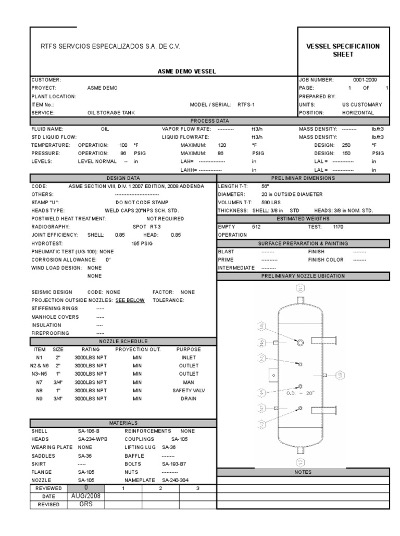
\includegraphics[width=0.5\textwidth]{images/vessel_specification.jpg}
    \caption{Vessel Specification Sheet \autocite{Itur}}
    \label{vessel_specification}
\end{figure}

\newpage


\section{The Automatic Identification System (AIS) dataset}

AIS (Automatic Identification System) was developed in the 1990s to enhance navigation safety and prevent ship collisions.
It allows ships equipped with AIS to communicate with each other and coastal authorities through VHF transmissions.
The International Maritime Organization (IMO) mandates that all international voyage ships above 300 gross tonnage and all passenger ships must have an AIS transmitter.
Governments and authorities in different nations also enforce AIS applications to improve safety and security.

\begin{figure}[h]
    \centering
    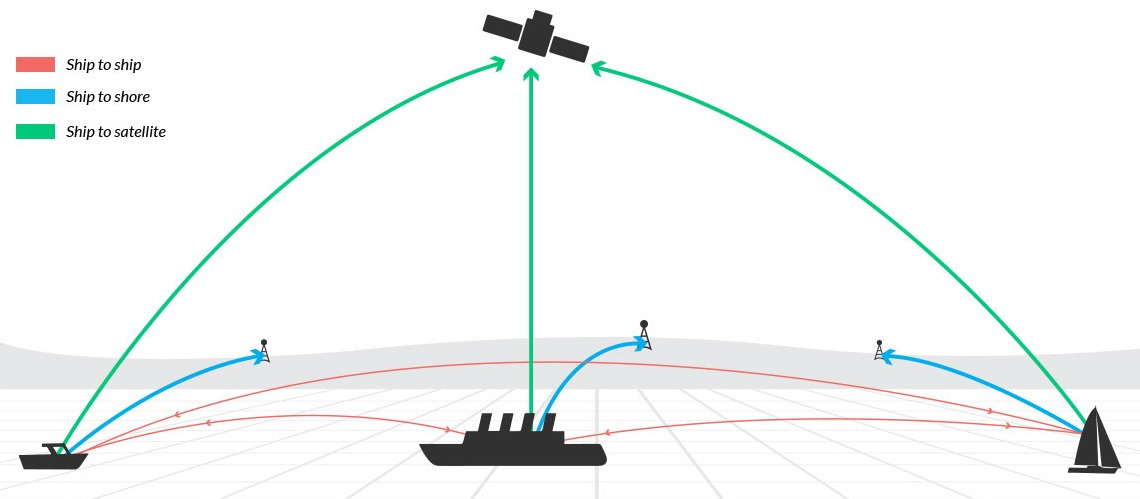
\includegraphics[width=0.7\textwidth]{images/ais.jpeg}
    \caption{Working of AIS}
    \label{ais}
\end{figure}

There are two types of AIS transceivers: Class A and Class B.
Class A transceivers broadcast more datafields and have higher reporting frequencies.
The information broadcasted by a Class A transceiver can be categorized into static information, dynamic information, and voyage-related information.
Dynamic information is automatically transmitted every 2-10 seconds when the ship is underway and every 3 minutes when anchored.
Static and voyage-related information are broadcasted every 6 minutes regardless of navigational status.
Class B transponders transmit a reduced set of data and have sparser reporting intervals compared to Class A transponders.


\begin{table}[ht]
    \centering
    \begin{tabular}{|l|l|p{0.5\linewidth}|}
        \hline
        \textbf{Data field}       & \textbf{Type} & \textbf{Description}                                                                      \\
        \hline
        AIS identity and location & Static        & Maritime Mobile Service Identity (MMSI) and the location of the system's antenna on board \\
        \hline
        Ship identity             & Static        & Ship name, IMO number, type, and call sign of the ship                                    \\
        \hline
        Ship size                 & Static        & Length and width of the ship                                                              \\
        \hline
        Ship position             & Dynamic       & Latitude and longitude (up to 0.0001 min accuracy)                                        \\
        \hline
        Speed                     & Dynamic       & Ranging from 0 knot to 102 knots (0.1 knot resolution)                                    \\
        \hline
        Rate of turn              & Dynamic       & Right or left (ranging from 0 to 720° per minute)                                         \\
        \hline
        Timestamp                 & Dynamic       & Timestamp of the message in UTC                                                           \\
        \hline
    \end{tabular}
    \caption{AIS message data fields \autocite{perez2009automatic}}
    \label{tab:ais_message}
\end{table}


Table \ref{tab:ais_message} shows the data fields transmitted by AIS messages.
Combining AIS data with other databases can provide additional information.
For example, port-to-port average speed can be calculated based on voyage distance and time stamps reported at the two ports.
Cargo weight can be estimated using draught and ship sizes. Technical ship specifications, such as DWT (deadweight tonnage), capacity, design speed, and design draught, can be obtained from fleet databases using the IMO number.
Port-to-port bunker consumption can be estimated based on speed, distance, and technical ship specifications like DWT and capacity \autocite{yang2019big}.


(Write more about the dataset source and how it is collected)



\section{AIS Trade Flow System}

AIS Trade Flow systems utilize data transmitted by vessels worldwide to furnish both real-time and historical insights into maritime trade operations \autocite{halden2019estimation}. 
The primary aim is to establish a framework that delineates trade activities between ports, leveraging AIS signals. 
Designating port areas within AIS Trade Flow systems is a multifaceted undertaking encompassing geographical and operational factors. 
From a geographical perspective, a port area is typically demarcated by a set of coordinates outlining the physical confines of the port and its adjacent waters. 
This encompassing region might encompass berths, anchorages, and at times, even approach channels. Identifying whether a ship resides within a port area often necessitates comparing its current AIS-reported coordinates with the established port boundaries. 
Should the ship's location fall within these boundaries, it's deemed situated within the port area. 
Nonetheless, the analysis transcends mere geographical coordinates. 
For instance, a ship might exist within a port's geographical bounds; 
however, if it's merely passing through without halting or participating in port operations, it might not qualify as being `in port` from an operational standpoint.

Addressing these intricacies, AIS Trade Flow systems frequently employ advanced algorithms to precisely ascertain port boundaries and classify vessel conduct. 
This assessment takes into account parameters like the vessel's velocity, heading, and historical behavioral trends. 
Through the integration of these diverse data facets, these systems can render an exceptionally precise portrayal of port undertakings and vessel trajectories. 
AF Code has constructed such a system by adhering to overarching principles, resulting in the creation of a dataset incorporating AIS signals alongside information about port visits, cargo loading, and unloading.



\begin{figure}[h]
    \centering
    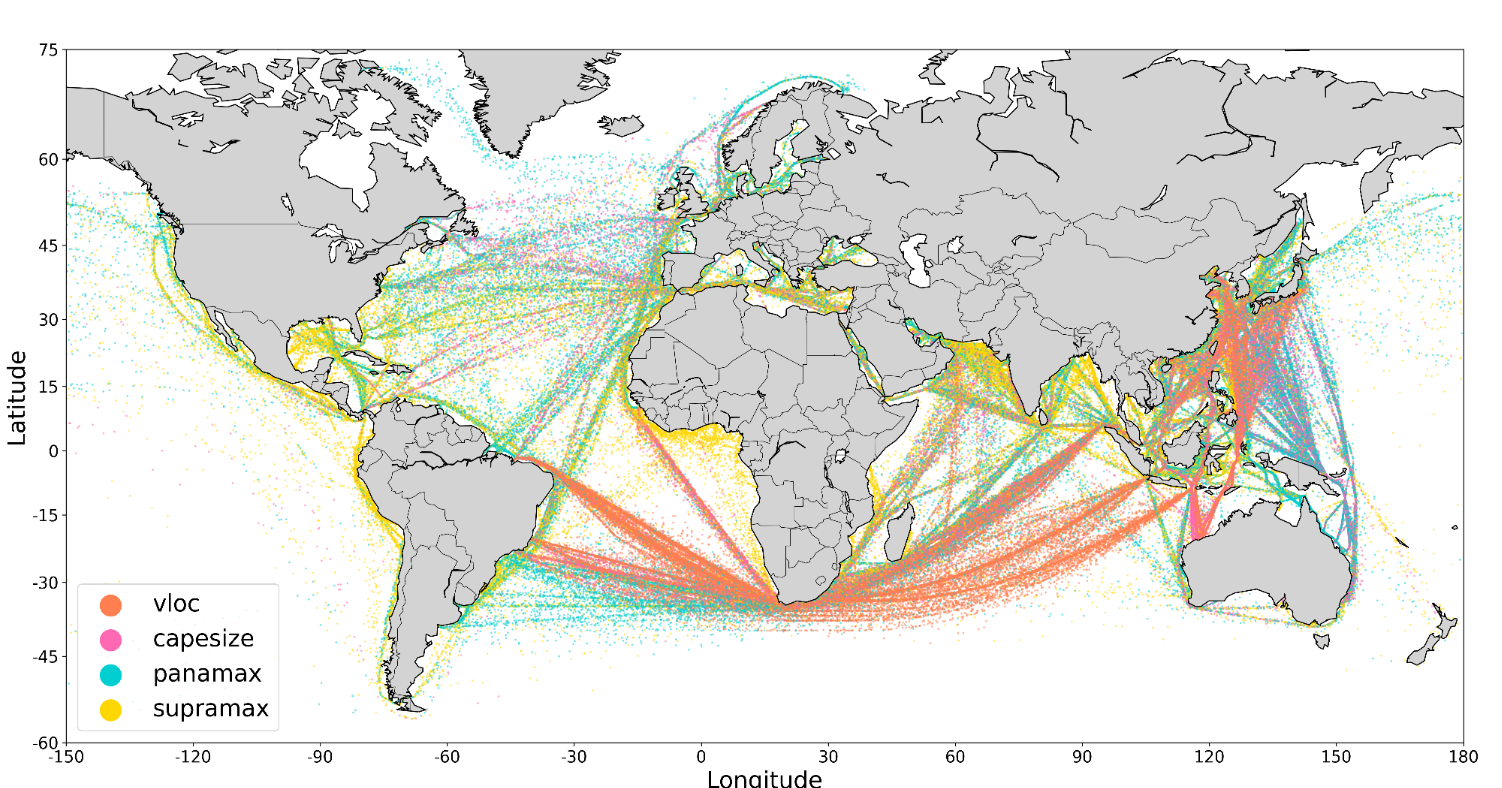
\includegraphics[width=0.7\textwidth]{images/tradeflow_system.png}
    \caption{Trade flow from 150,000 AIS sampled signals.}
    \label{tradeflow_system}
\end{figure}

To achive this, the AIS data is processed to identify port-to-port voyages and then stored them in a database based on segments as shown in the Figure \ref{ais_processing}

\begin{figure}[h]
    \centering
    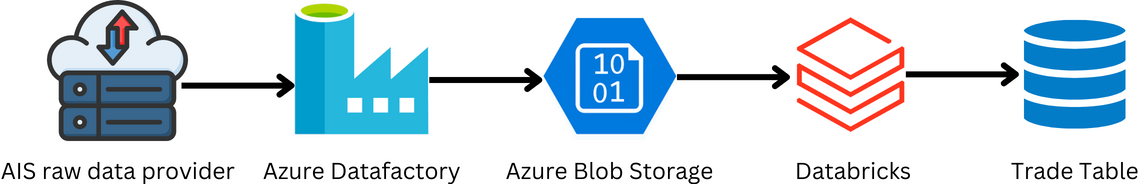
\includegraphics[width=0.8\textwidth]{images/ais_processing.png}
    \caption{AIS Raw Data Processing}
    \label{ais_processing}
\end{figure}

\subsection{Vessel Voyages}

Trade flow systems are designed to identify port-to-port voyages. 
Each of this voyages is either Laden voyage or Ballast voyage from one port to another. 
At port vessel can load or unload cargo or just refuel and continue to another port.
It is important to determine port stops and port area to identify the type of voyage.
This section will describe how these voyages are identified and classified. 


\subsubsection{Laden Voyages}

The laden voyage concept centers on cargo movement, distinct from the vessel's own traversal. 
This characterization holds particular significance in evaluating logistical chains and cargo dynamics within maritime transportation. 
A laden voyage pertains to the route spanning from the cargo's loading point at the departure port to its unloading point at the arrival port. 


\subsubsection{Ballast Voyages}

The ballast voyage concept centers on the vessel's movement without cargo, contrasting with its movement when laden. 
A ballast voyage is characterized as the route from the port of cargo unloading, serving as the departure port, to the port of cargo loading, functioning as the arrival port.

\subsection{Port Stop and Port Area}

The initial key phase involves obtaining the coordinates of the targeted port and subsequently establishing a polygon encompassing its vicinity. 
The overarching approach revolves around quantifying unique visits within this polygon, using a geo-fence strategy. 
Given the utilization of S-AIS data, there exist temporal intervals during which satellites may not receive ship messages due to blind zones. 
This introduces the potential for ships to enter and exit the designated port area without satellite detection. 
To mitigate this, a larger polygon around the port can decrease the likelihood of overlooked visits. However, such an expansive polygon could result in the inclusion of vessels merely passing through, particularly if the port is positioned near a major shipping route. 
Hence, the ideal polygon size is contingent on the port's location, it should be sizable enough to capture all visits yet sufficiently compact to exclude vessels in transit. 
This is illustrated by Figure \ref{port_area}, showcasing LNG terminals in Trinidad and Algeria enclosed by identical polygons.
Visual inspection reveals message flow towards the port in Trinidad (5.4a) and a substantial portion of vessel flow bypassing the port in Algeria (5.4b). 
Additionally, supplementary criteria like capping maximum speed and requiring navigational statuses of $anchored$ or $moored$ can be incorporated to ensure vessels are genuinely engaged in loading activities \autocite{halden2019estimation}.

\begin{figure}[h]
    \centering
    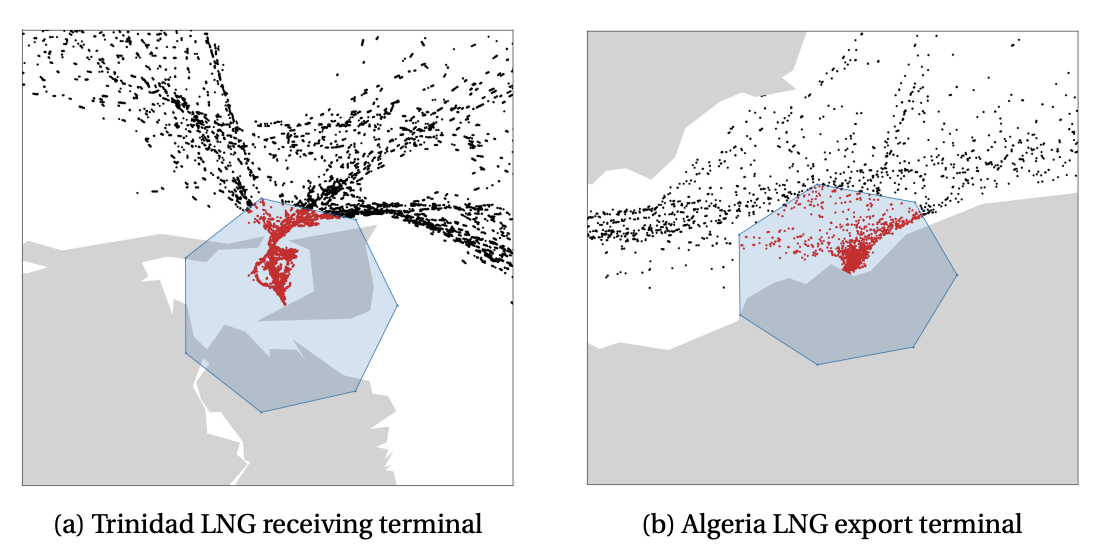
\includegraphics[width=0.8\textwidth]{images/port_area.png}
    \caption{Port Area}
    \label{port_area}
\end{figure}

By using the trade flow system described in this section, we can figure out the trades made by ships in 2022. 
If we assume that these ships will continue with the same trading patterns in 2023, we can use the trade data to make an estimate of emissions for 2023.


\chapter{Data Analysis Techniques}

In this section, we will use tradeflow data for the year 2022, along with specifications from the IHS dataset, to perform data analysis.

\section{Tools}

To perform data analysis, we will utilize the following tools:

\begin{itemize}
    \item Python
    \item Databricks
    \item Apache Spark
    \item MSSQL
    \item Pandas
    \item Astrup Fearnleys Code Emission Calculator API
\end{itemize}

\subsection{Databricks}

Databricks is a leading platform for big data analysis, specifically designed to handle \newline large-scale datasets efficiently and effectively.
Leveraging Apache Spark as its core engine, Databricks provides a distributed computing framework that enables processing massive volumes of data in parallel across multiple nodes.
This distributed architecture allows for significant performance improvements, reducing the time it takes to process and analyze big data compared to traditional approaches.
With its ability to handle both batch and real-time data processing, Databricks empowers data engineers and analysts to extract valuable insights from vast datasets, enabling them to make data-driven decisions at scale.

One of the key advantages of using Databricks for big data analysis is its ease of use and collaborative features.
The platform offers interactive notebooks (Figure \ref{databricks_notebook})  that allow data professionals to write, execute, and share code seamlessly.
This enables collaborative data exploration and simplifies the iterative process of data analysis and model development.
Moreover, Databricks provides a rich set of built-in libraries and integrations with popular big data tools and machine learning frameworks, streamlining the development and deployment of complex data pipelines and advanced analytical models.
By abstracting the complexities of distributed data processing, Databricks empowers data teams to focus on the analysis and interpretation of results, accelerating the time-to-insight for big data projects and ultimately driving business growth and innovation.
One of the key benefits of using Databricks for big data analysis is its ability to handle large volumes of data with ease.
Whether you're working with terabytes, petabytes, or even exabytes of data, Databricks can scale to meet your needs without sacrificing performance or reliability.
This makes it an ideal solution for organizations looking to perform complex big data analysis tasks, such as machine learning, data warehousing, and real-time streaming analytics \autocite{databricksDataLakehouse}.

\begin{figure}[ht]
    \centering
    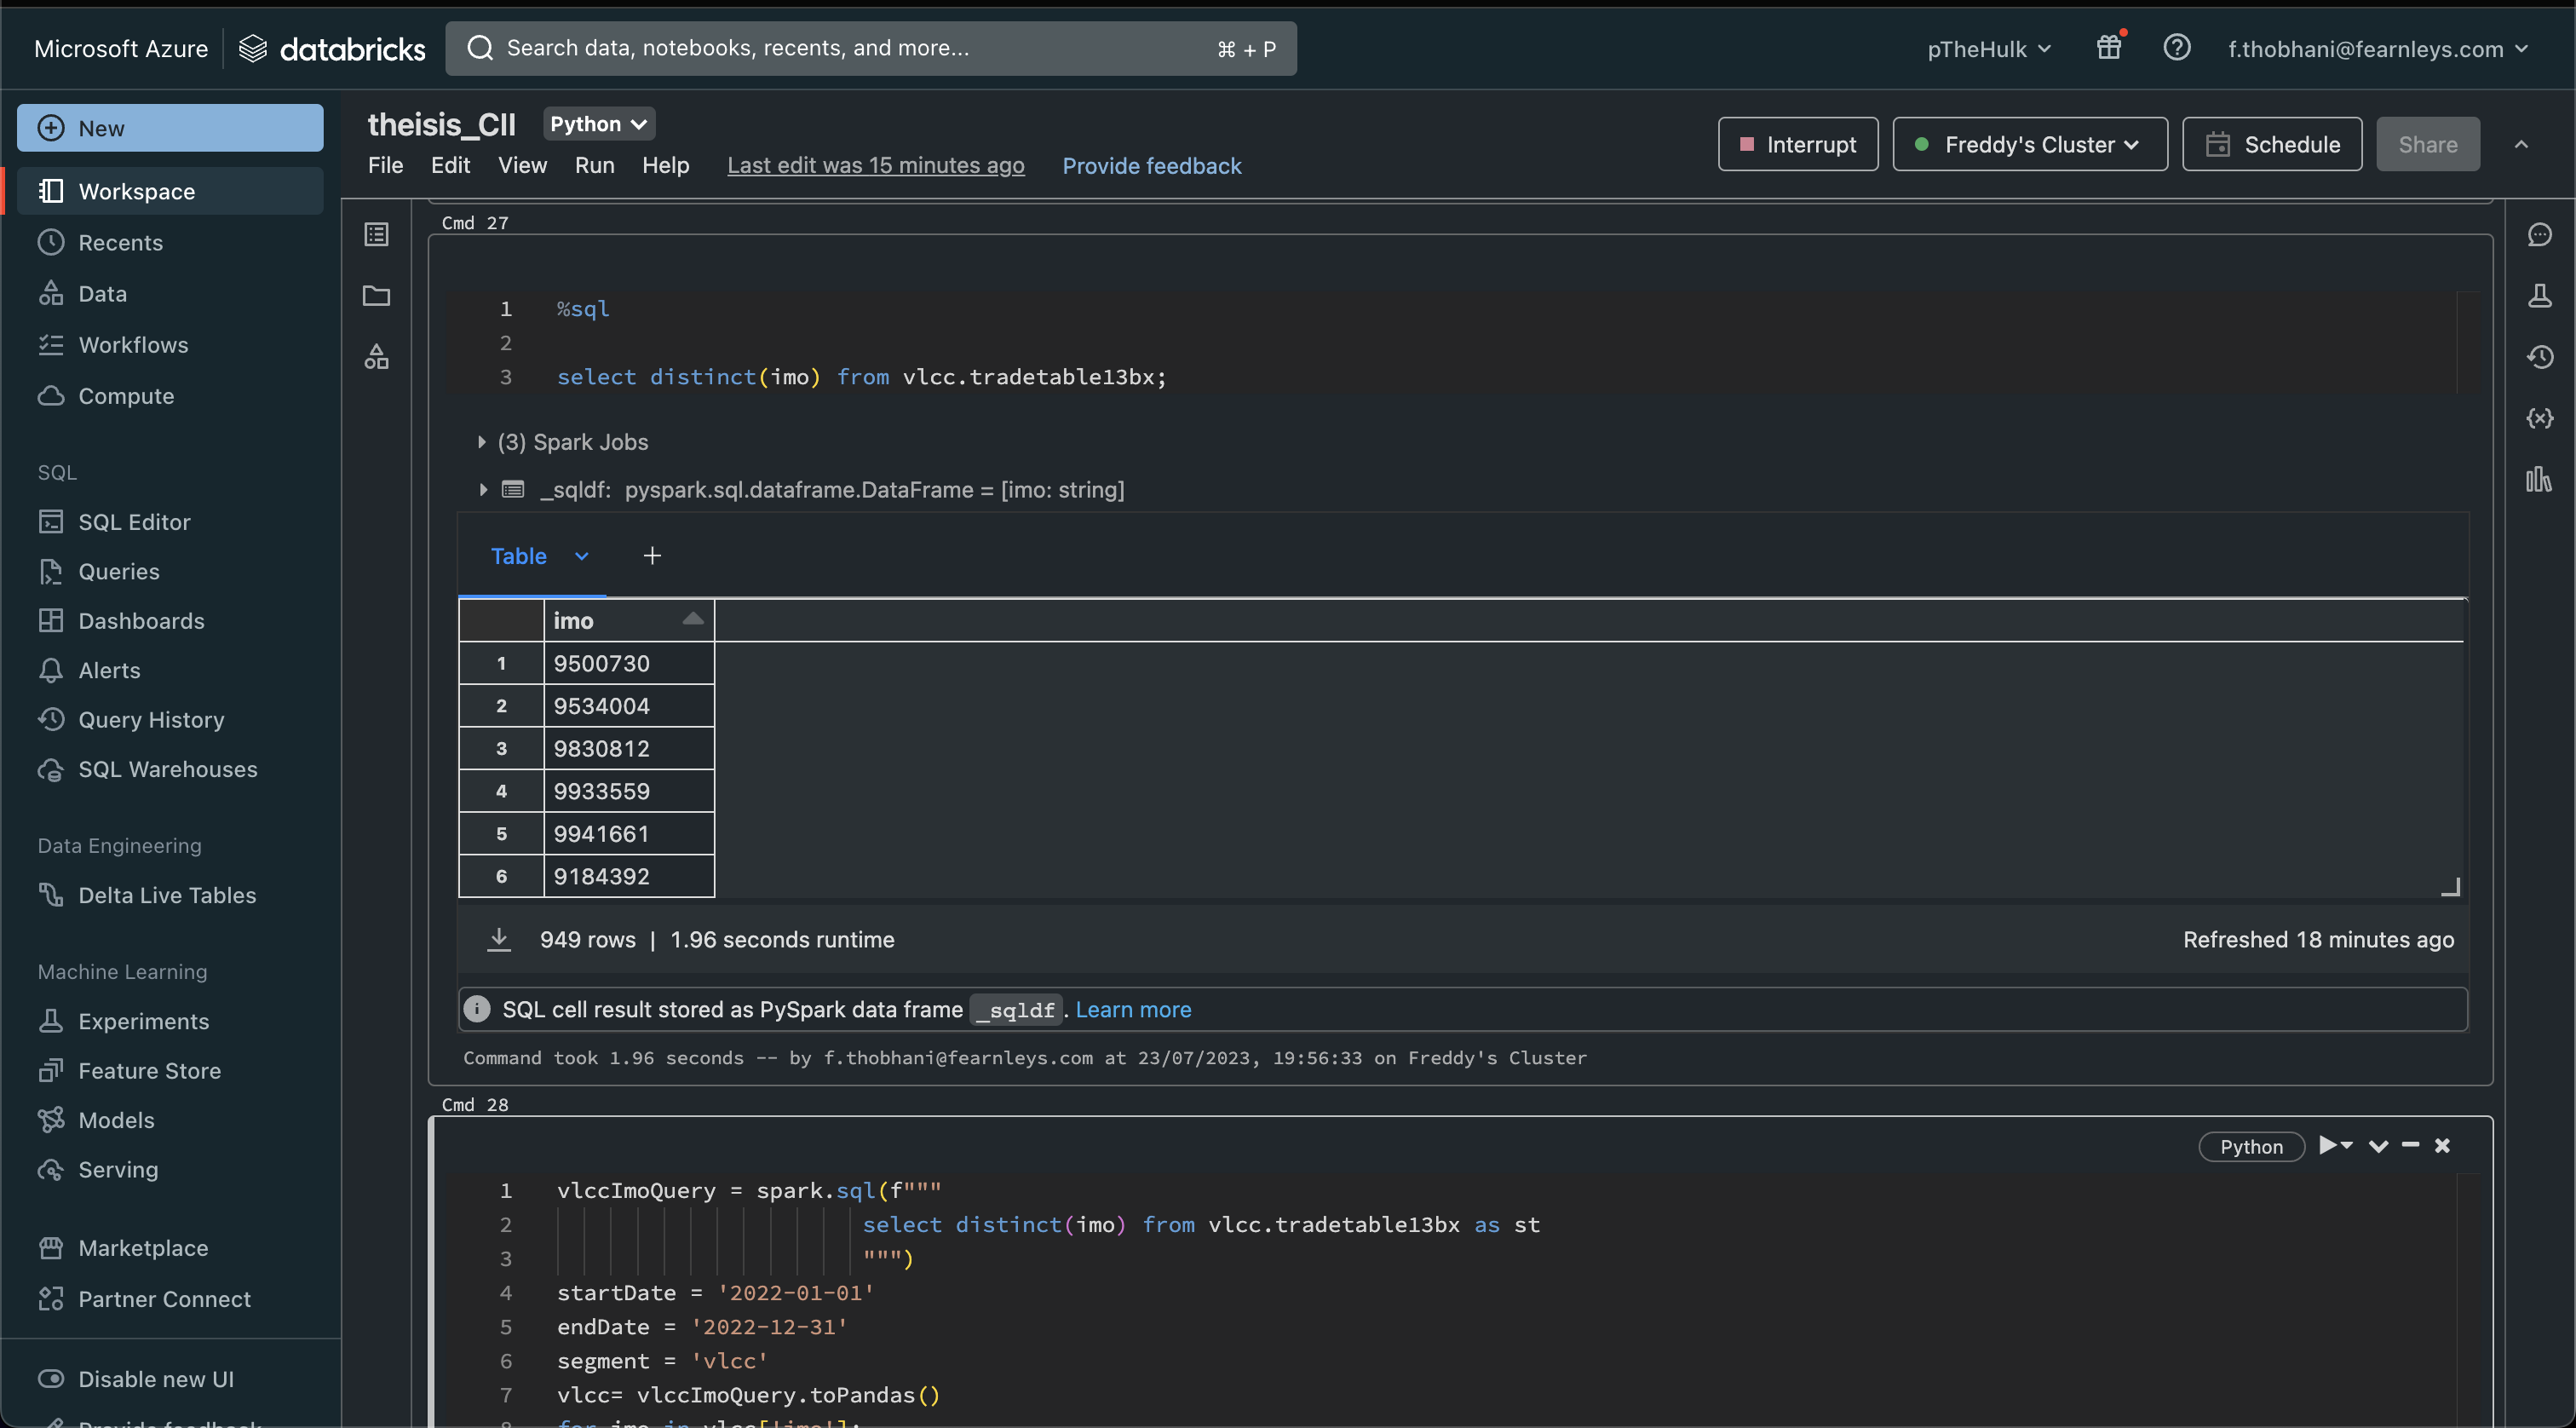
\includegraphics[width=1\textwidth]{images/databricks_notebook.png}
    \caption{Databricks Notebook}
    \label{databricks_notebook}
\end{figure}

Overall, Databricks is a highly capable platform for big data analysis that is well-suited to a wide range of use cases, from simple data processing tasks to complex machine learning and statistical analysis.

The entire analysis will be conducted on Databricks with the following configuration:

\begin{itemize}
    \item Databricks Runtime Version: 11.3 LTS (includes Apache Spark 3.3.0, Scala 2.12)
    \item 8GB Memory, 4 Cores with 1 driver and 1 worker node.
    \item Python 3
    \item Elastic Disk
\end{itemize}

\begin{figure}[ht]
    \centering
    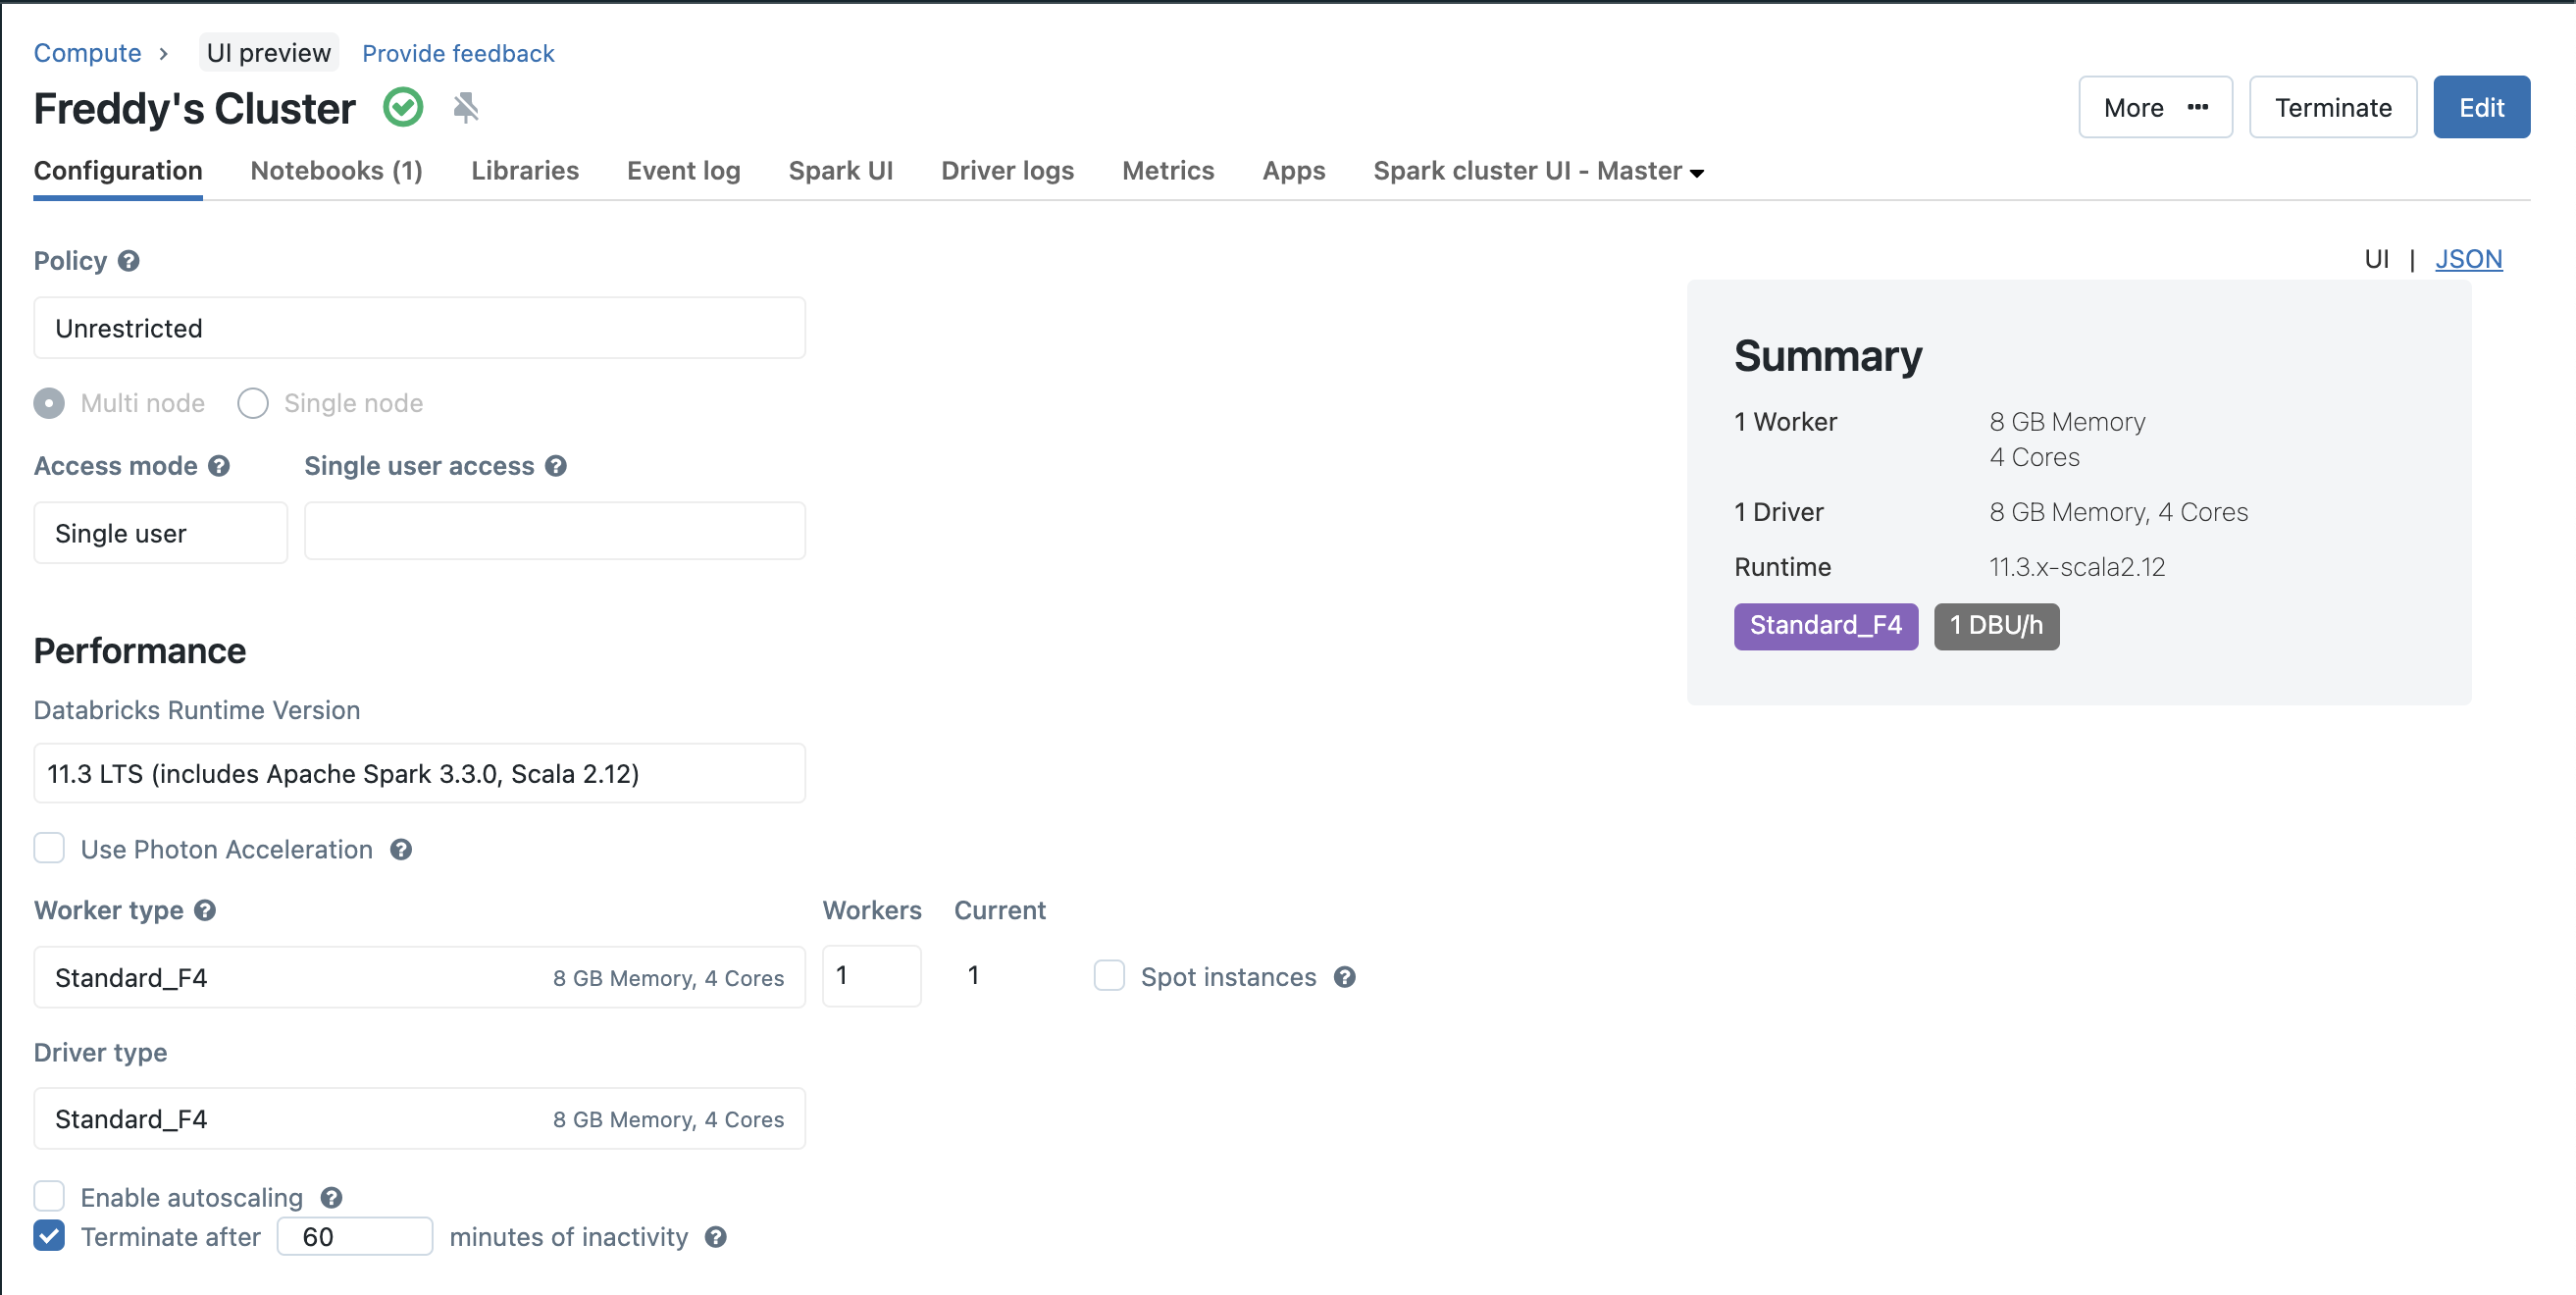
\includegraphics[width=1\textwidth]{images/databricks_configuration.png}
    \caption{Databricks Configuration}
    \label{databricks_configuration}
\end{figure}


\subsection{Apache Spark}

Apache Spark is an open-source distributed computing framework designed for processing and analyzing large-scale datasets in a highly efficient and parallel manner.
It provides a unified platform that supports various data processing tasks, including batch processing, real-time streaming, machine learning, and graph processing.
Spark's core abstraction is a resilient distributed dataset (RDD), which allows data to be distributed across multiple nodes in a cluster, enabling data processing operations to be executed in parallel \autocite{apacheSpark}.

Databricks leverages Apache Spark as its underlying engine to offer a powerful and scalable data analytics platform.
By integrating Spark into its infrastructure, Databricks provides users with a seamless and interactive environment for collaborative data engineering and data science tasks.
Databricks' interactive notebooks allow data professionals to write and execute Spark-based code, making it easier to perform data manipulations, transformations, and analysis in real-time.
The platform also offers support for various programming languages such as Python, Scala, R, and SQL, providing users with flexibility and familiarity in their preferred language.

Furthermore, Databricks enhances Apache Spark by providing additional features and optimizations to improve performance and ease of use.
The platform offers auto-scaling capabilities, enabling resources to be automatically allocated and released based on the workload demand, ensuring optimal performance and cost-efficiency.
Databricks also provides built-in libraries and tools that simplify complex tasks such as machine learning and data visualization, allowing data scientists to focus on building and deploying advanced analytical models with ease.

In summary, Apache Spark forms the backbone of Databricks, enabling the platform to handle large-scale datasets efficiently and deliver a collaborative and user-friendly environment for data analysis, making it a popular choice for organizations seeking to harness the potential of big data analytics.

\begin{figure}[h]
    \centering
    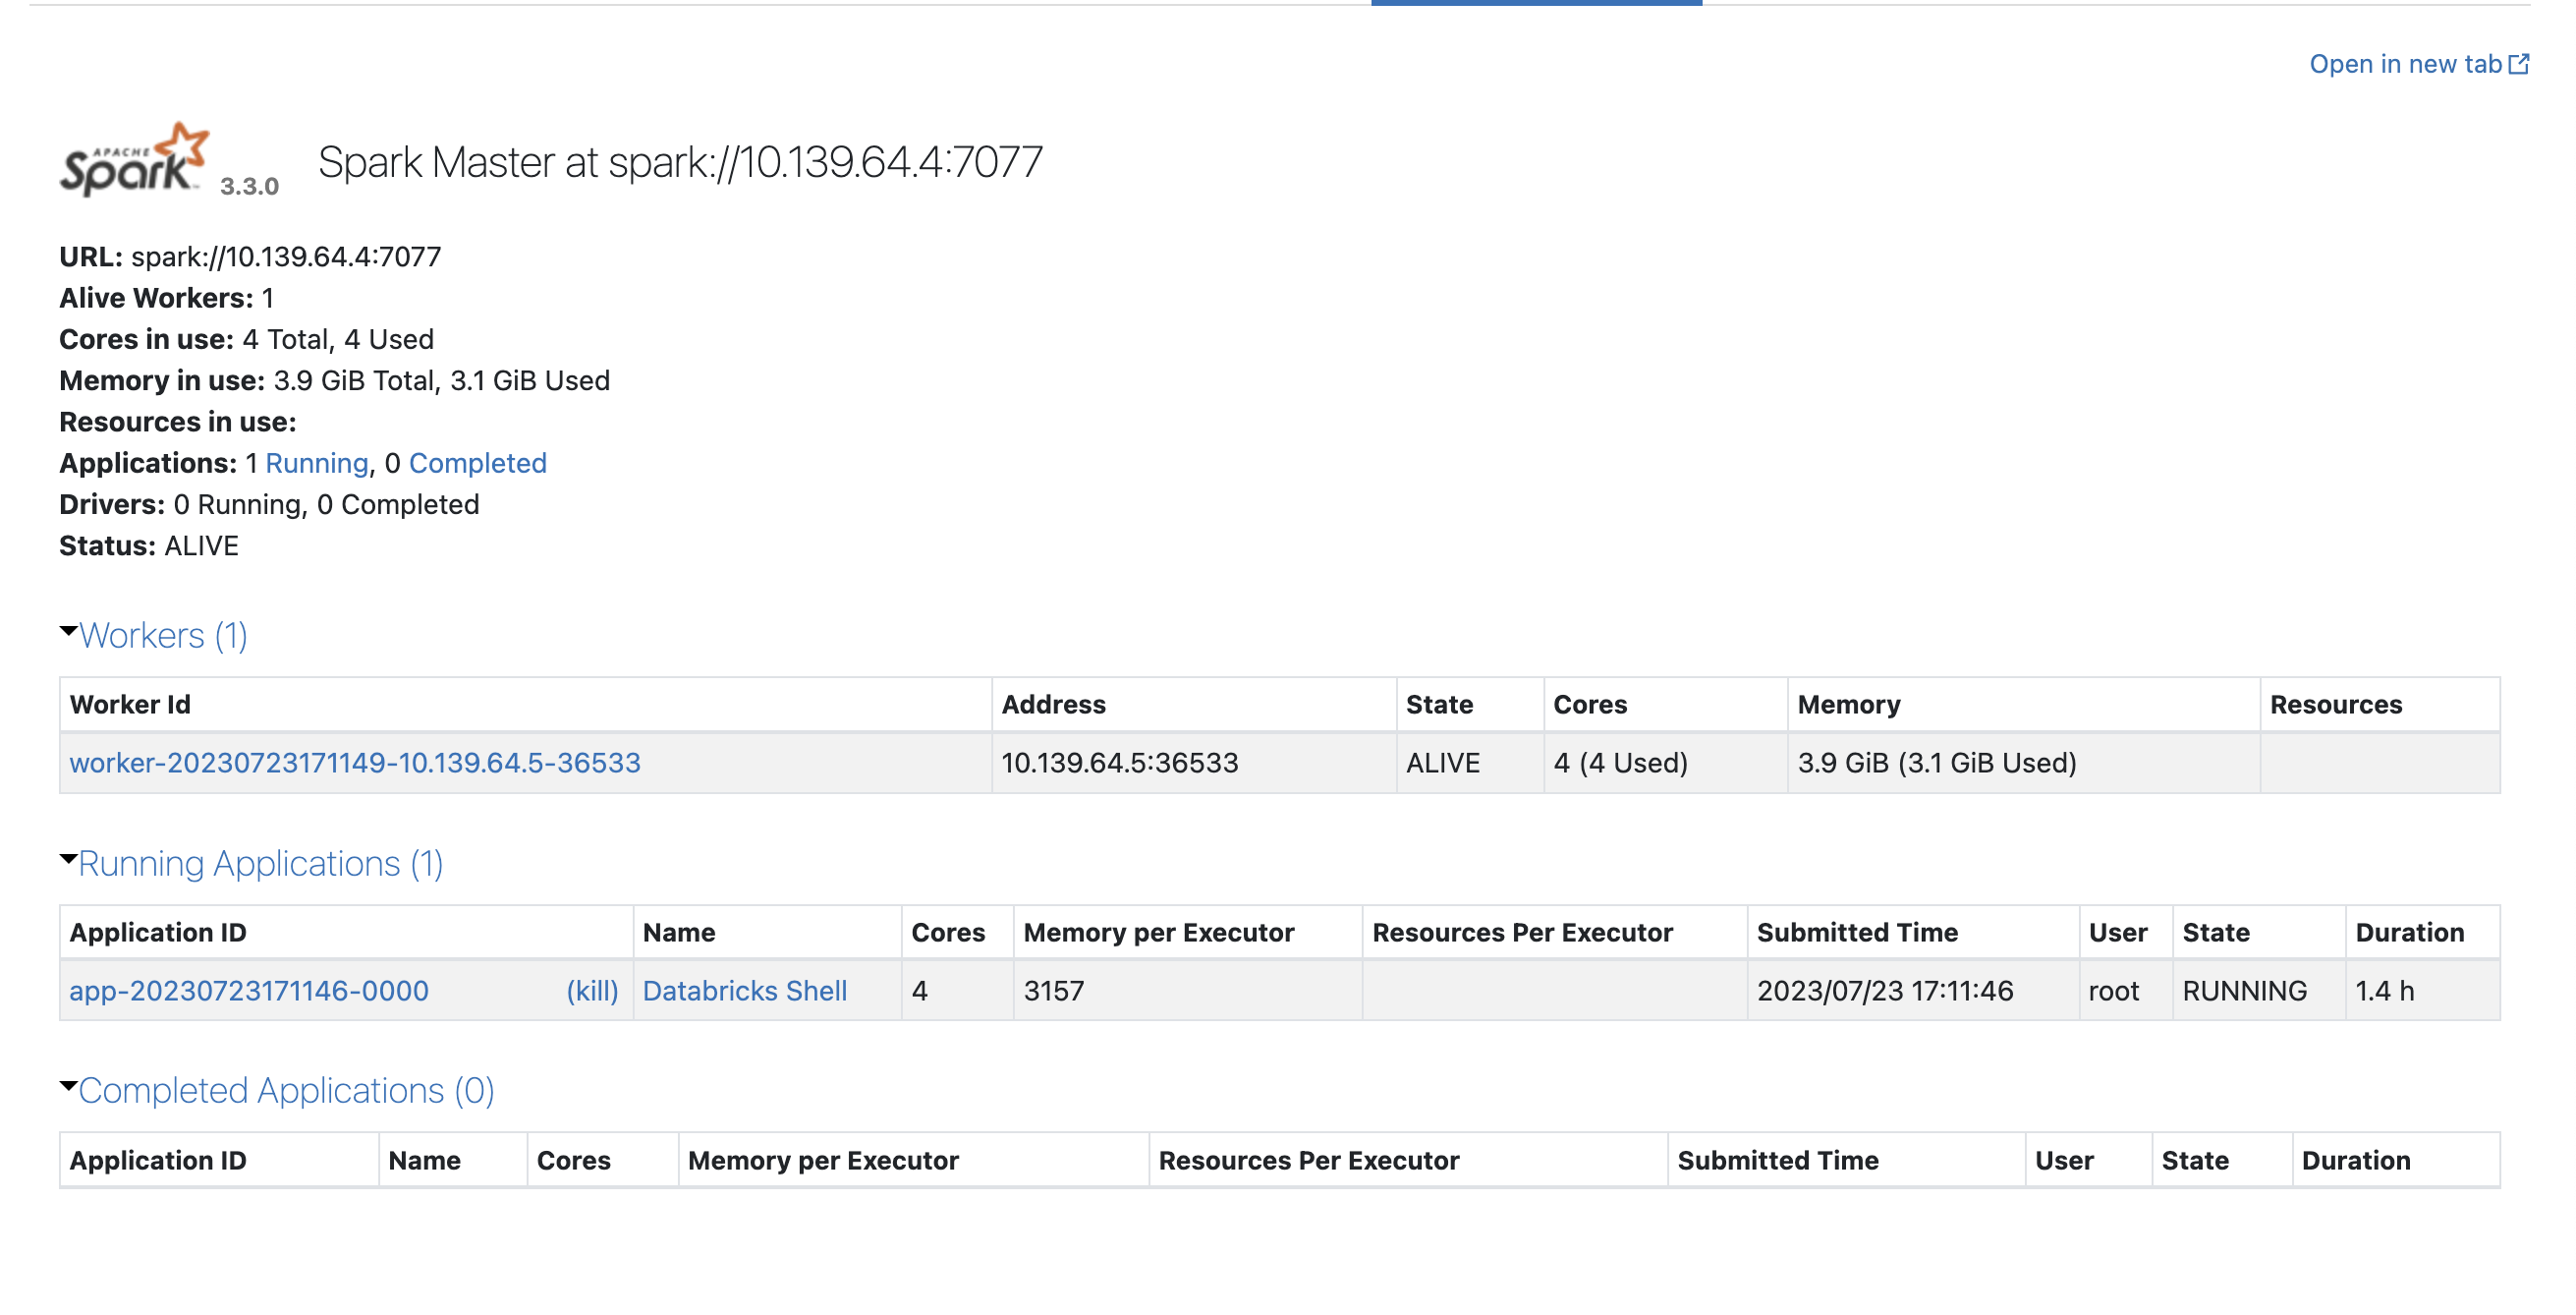
\includegraphics[width=1\textwidth]{images/spark_config.png}
    \caption{Apache Spark Configuration}
    \label{spark_config}
\end{figure}

\subsection{Astrup Fearnleys Code Emission Calculator API}

Astrup Fearnleys Code Emission Calculator API is a service that provides a simple interface for calculating the emissions of a given vessel.
The API is built on top of the Astrup Fearnleys Code Emission Calculator, It is internal tool developed to provide a simple interface for calculating the emissions of a given vessel for researchers.

It requires the following parameters to be passed as a input:

\newpage

\begin{table}[h]
    \centering
    \begin{tabular}{|p{0.2\linewidth}|p{0.2\linewidth}|p{0.5\linewidth}|}
        \hline
        \textbf{Parameter}  & \textbf{Type} & \textbf{Description}                                                                                                          \\
        \hline
        imo                 & integer       & IMO of a ship that will require emission calculations.                                                                        \\
        \hline
        avg\_speed\_kn      & number        & The vessel's intended average sailing speed in knots on the route. Optional if duration\_h is given.                          \\
        \hline
        distance\_nm        & number        & Expected length of the voyage in Nautical Miles.                                                                              \\
        \hline
        cargo\_unit         & string        & Cargo unit used to submit cargo\_amt. Currently, the only possible value is tons. Used to calculate EEOI and transport\_work. \\
        \hline
        cargo\_amt          & number        & Amount of cargo the ship is carrying (in the given cargo\_unit). Used to calculate EEOI and transport\_work.                  \\
        \hline
        me\_fuel\_type      & string        & Fuel type to be considered for the main engine consumption for the emissions estimate. Overwriting the model assumption.      \\
        \hline
        ae\_fuel\_type      & string        & Fuel type to be considered for the auxiliary engine consumption for the emissions estimate. Overwriting the model assumption. \\
        \hline
        boiler\_fuel\_type  & string        & Fuel type to be considered for the boiler consumption for the emissions estimate. Overwriting the model assumption.           \\
        \hline
        duration\_h         & number        & Expected duration of the voyage in hours. Optional if avg\_speed\_kn is given.                                                \\
        \hline
        load\_cond          & string        & Loading condition of the vessel to be considered in the power estimation.                                                     \\
        \hline
        me\_co2\_factor     & number        & CO2 factor for the main engine fuel. Main engine fuel type must be specified.                                                 \\
        \hline
        ae\_co2\_factor     & number        & CO2 factor for the auxiliary engine fuel. Auxiliary engine fuel type must be specified.                                       \\
        \hline
        boiler\_co2\_factor & number        & CO2 factor for the boiler engine fuel. Boiler engine fuel type must be specified.                                             \\
        \hline
    \end{tabular}
    \caption{Request Parameters for Emission Calculations}
    \label{tab:request-parameters}
\end{table}

In return, it provides the JSON output in following format:


\begin{lstlisting}[language=JSON, caption=JSON output format from emission api]
    {
      "imo": 1234567,
      "avg_speed_kn": 10.045,
      "load_cond": "ballast",
      "cargo_unit": "tons",
      "cargo_amt": 544385.543,
      "me_fuel_type": "MGO",
      "ae_fuel_type": "MGO",
      "boiler_fuel_type": "MGO",
      "duration_h": 354.5,
      "me_fuel_cons_metric_metric_tons": 0.1,
      "ae_fuel_cons_metric_metric_tons": 0.1,
      "boiler_fuel_cons_metric_metric_tons": 0.1,
      "total_co2_emission_metric_tons": 0.1,
      "total_so2_emission_metric_tons": 0.1,
      "total_particulate_matter_emission_metric_tons": 0.1,
      "total_nox_emission_metric_tons": 0.1,
      "total_nmvoc_emission_metric_tons": 0.1,
      "total_ch4_emission_metric_tons": 0.1,
      "total_n2o_emission_metric_tons": 0.1,
      "total_co_emission_metric_tons": 0.1,
      "total_black_carbon_emission_metric_tons": 0.1,
      "total_organic_carbon_emission_metric_tons": 0.1,
      "transport_work": 0.1,
      "eeoi": 0.1,
      "me_co2_factor": 2.1,
      "ParamValidation": {
        "status": "OK"
      },
      "LimitMessage": {
        "message_description": "You are within your call limit"
      }
    }
    \end{lstlisting}



\section{Methodology}


In this section, using trade flow data for the year 2022, along with specifications from the IHS dataset, we will perform data analysis.

Tradetable data is available in the trade flow dataset. For each segments there is trade flow and therefore we will have to perform the analysis for each segment separately.

The steps involved in the analysis are as follows:

\begin{figure}[h]
    \centering
    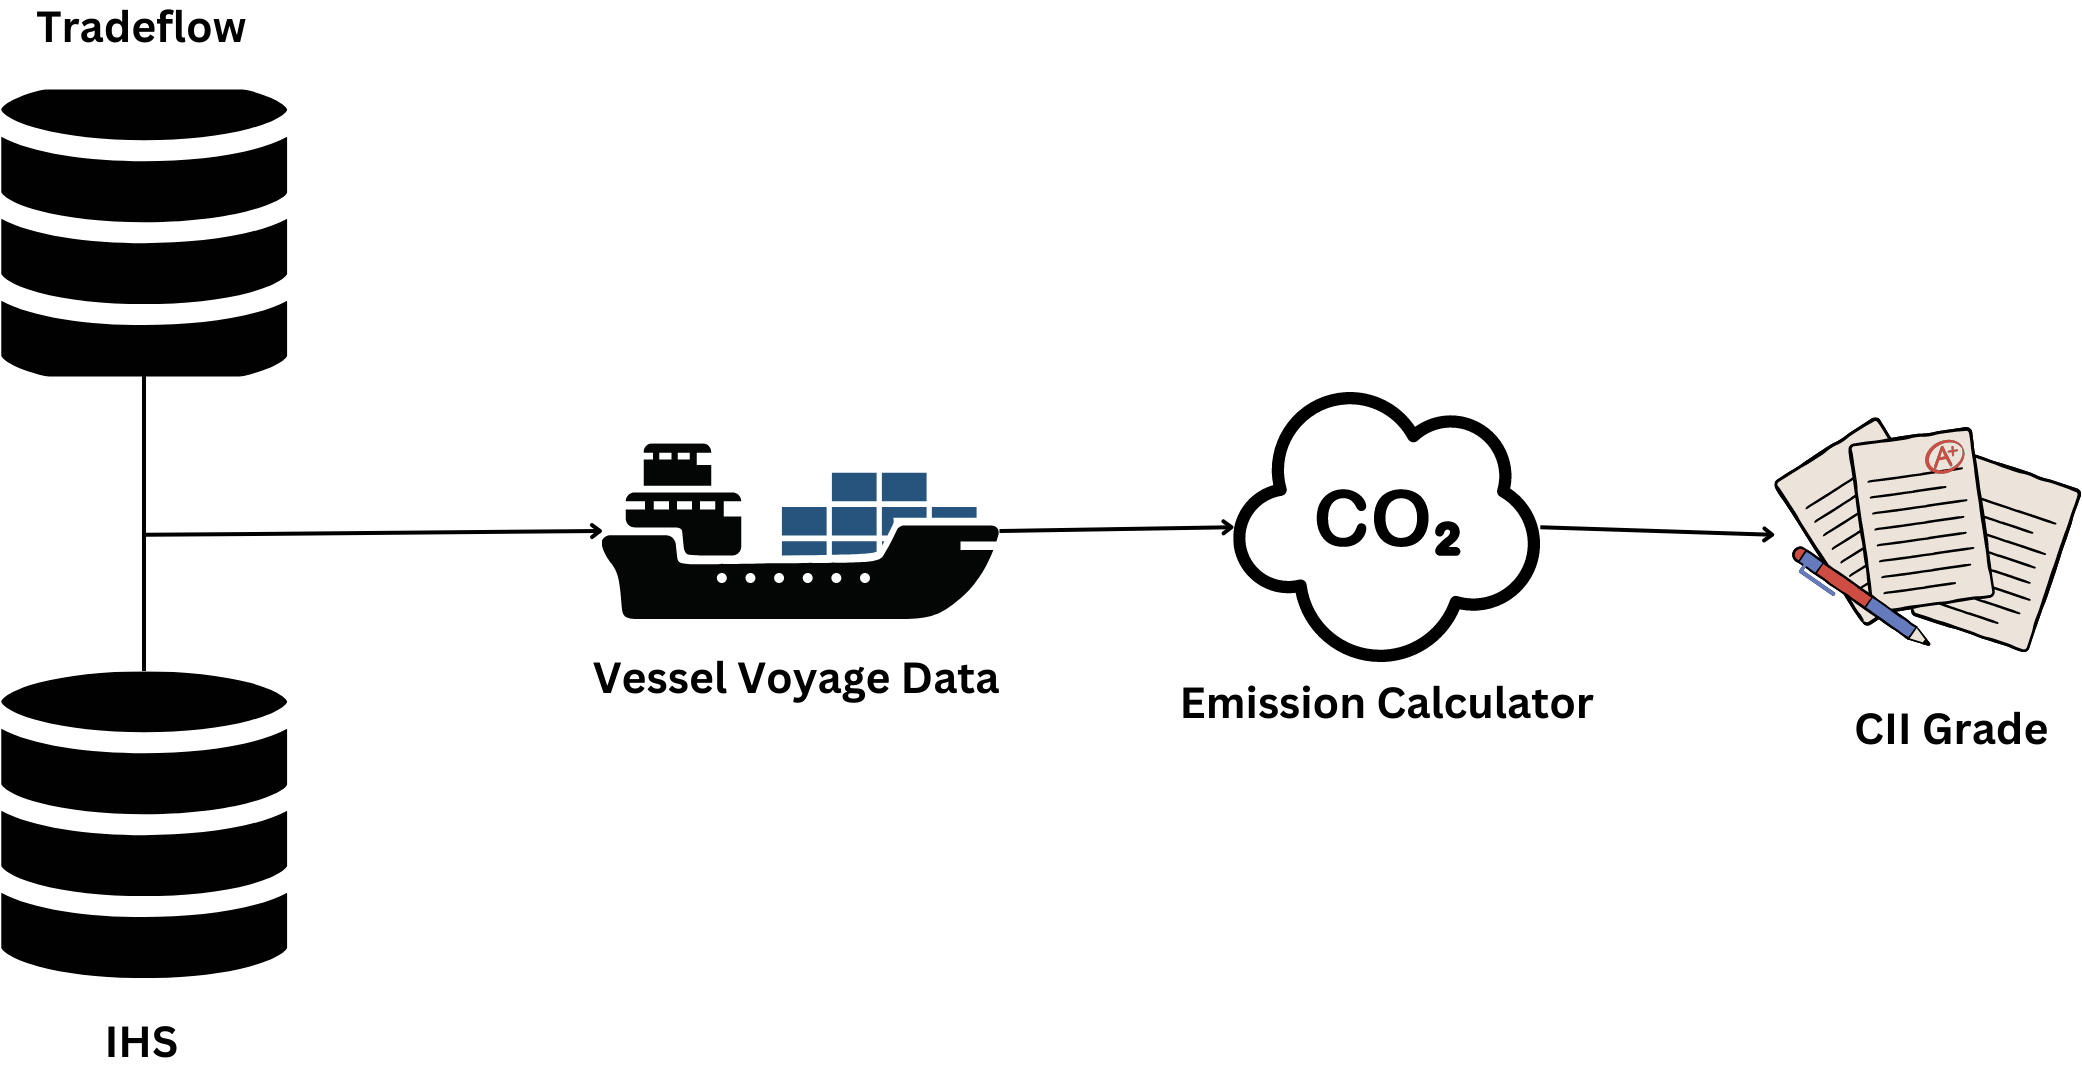
\includegraphics[width=0.5\textwidth]{images/methodlogy.png}
    \caption{Methodology Overview}
    \label{methodlogy}
\end{figure}

\newpage

\subsubsection{1. Getting distinct IMO numbers from trade flow}

Distinct IMO (International Maritime Organization) numbers were obtained from the trade flow dataset by querying the texttt{imo} column. 
This process helped in identifying all the unique ships present in the dataset, forming the foundation for further analysis.


\subsubsection{2. Getting necessary information for each IMO number from IHS and trade flow}

For each distinct IMO number identified in the previous step, the IHS dataset was queried or joined with trade flow to gather relevant information about each ship. 
This included details such as specifications, fuel type, engine types, and more. 
The process consisted of the following steps:

\begin{itemize}
    \item \textbf{Estimating Cargo Based on Draught:} Cargo was estimated using the draught noted on ports and the maximum draught from the IHS dataset. This allowed for an understanding of the cargo load for different vessels.
    
    \item \textbf{Determining Laden or Ballast Trade Flows:} The trade flows were categorized into laden or ballast based on the ballast threshold percentage from segment parameters. This categorization assisted in differentiating the vessel's operational conditions.
    
    \item \textbf{Converting to Pandas DataFrame:} The obtained shipTrade data was converted into a Pandas DataFrame, facilitating further processing and analysis.
    
    \item \textbf{Dividing into DataFrames for Laden and Ballast Trade Flows:} The trade data was divided into separate DataFrames for laden and ballast trade flows. This segmentation enabled focused analysis on different operational conditions.
    
    \item \textbf{Extracting Information on Distance, Time, and Average Speed:} Information such as distance, time, and average speed was extracted for both ballast and laden trade flows. These parameters provided insights into the efficiency and operation of the vessels.
    
    \item \textbf{Calculating Cargo:} The total cargo was calculated based on laden trade data, contributing to the overall understanding of the vessels' capacity and utilization.
\end{itemize}



\subsubsection{3. Cleaning data}

Data cleaning is a critical step in the methodology, ensuring that the dataset is ready for analysis. This involves handling missing values, removing duplicates, standardizing units, and correcting any inconsistencies. Specific aspects of the data cleaning process included:


\begin{itemize}
    \item \textbf{Handling Missing Speed Values:} In some cases, the average speed determined from AIS (Automatic Identification System) data might be missing or unusually high for specific trade flows. To address this, the distance and time values were used to calculate the average speed, ensuring that the analysis was based on consistent and realistic speed data.
    
    \item \textbf{Excluding Trades with Missing Distance:} Any trades with missing average distance values were excluded from the analysis. This helped maintain the integrity and accuracy of the dataset.
    
\end{itemize}


Sometimes for certain trades average distance was missing, this trades were excluded.

\subsubsection{4. Calculating emissions for laden and ballast tradeflows.}

The calculation of emissions for laden and ballast trade flows was a central component of the methodology. Utilizing the information extracted in the previous steps, the emissions were calculated using the AFC (Automated Flight Control) emission calculator API. Here's how the process was executed:

\begin{itemize}
    \item \textbf{Emission Calculation Function:} A specific function, getEmission, was employed to calculate emissions. This function took essential parameters like IMO number, cargo amount, distance, load condition, and estimated speed as input.
    
    \item \textbf{API Request:} The function made a request to the AFC emission calculator API, passing the required parameters. The response from the API included detailed emission data, providing insights into various emission aspects such as CO2, SO2, NO2, and others.
    \item 
    \item \textbf{Error Handling:} The process included robust error handling to manage any issues with the API request, ensuring that the analysis was not disrupted by unexpected errors or inconsistencies.
    
    
\end{itemize}

\subsubsection{5. Calculating CII, CII required, and CII reference.}

Carbon Intensity Indicator (CII) is calculated as the ratio of emissions (CO\textsubscript{2}) to transport work (distance traveled $\times$ cargo amount). CII required is based on regulatory standards, while CII reference can be derived from historical data or benchmarks. Calculate these indicators for each trade flow using the emission data and transport work values.

CII reference is calculated using the following formula:

\begin{equation}
    CII_{\text{ref}} = a \cdot \text{Capacity}^{-C}
\end{equation}

where $a$ and $C$ are constants according to Figure \ref{cii_ref_constant}, and Capacity is the deadweight of the ship.

\begin{figure}[h]
    \centering
    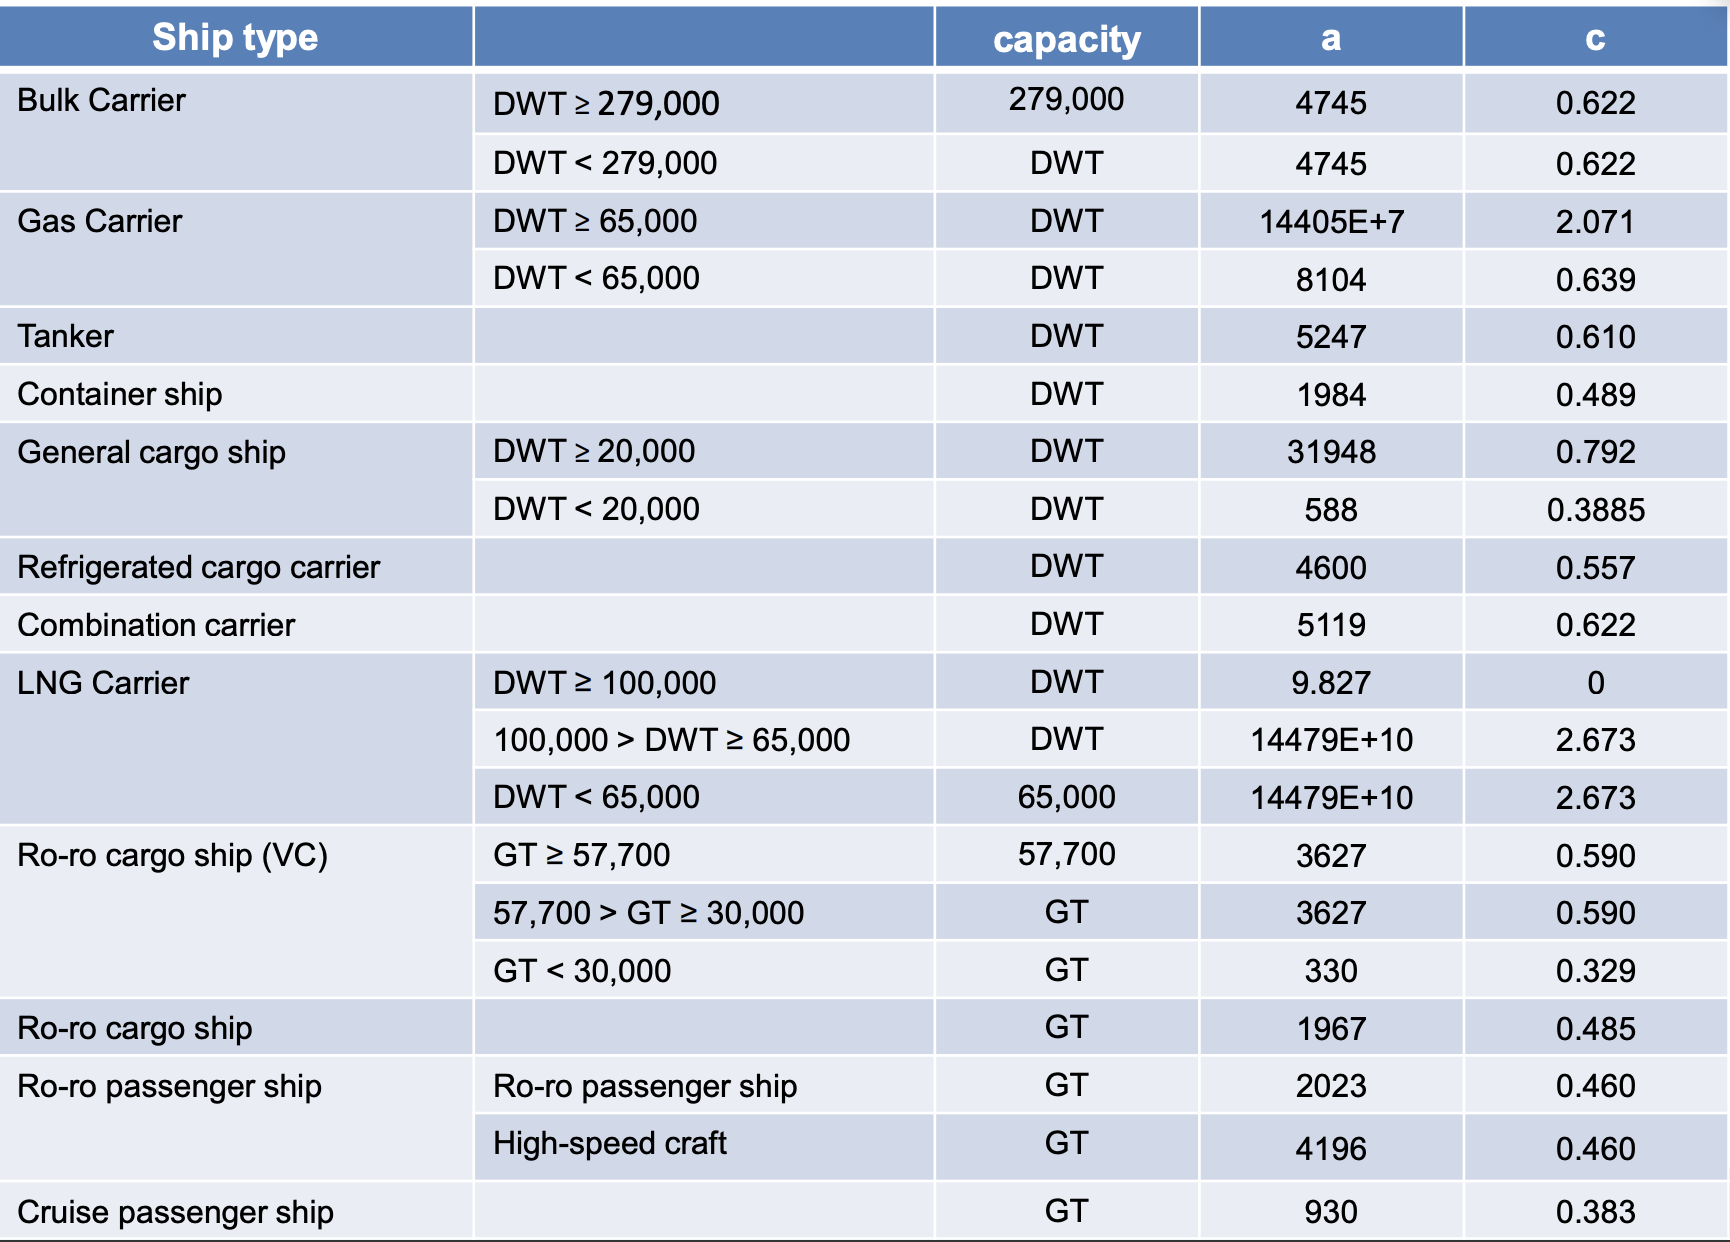
\includegraphics[width=1\textwidth]{images/cii_ref_constant.png}
    \caption{$a$ and $C$ constants}
    \label{cii_ref_constant}
\end{figure}

CII required can be calculated using the following formula:

\begin{equation}
    \text{Requited CII} = \left( \frac{100 -Z}{100}\right) \times \text{CIIRef}
    \label{cii_required}
\end{equation}

In Equation 5.2, the reduction factor Z represents the initial value of 5\% in the year 2023,
with an annual increment of 2\%. Additionally, for the years 2027 to 2030,
the Z factors are subject to enhancement and refinement, guided by the evaluation of the short-term measure's effectiveness.

\newpage

\begin{table}[htbp]
    \centering
    \begin{tabular}{cc}
        \toprule
        Year & Reduction Factor (Z) \\
        \midrule
        2023 & 5\%                  \\
        2024 & 7\%                  \\
        2025 & 9\%                  \\
        2026 & 11\%                 \\
        2027 & **                   \\
        2028 & **                   \\
        2029 & **                   \\
        2030 & **                   \\
        \bottomrule
    \end{tabular}
    \caption{Reduction Factors Over the Years}
    \label{tab:reduction-factors}
\end{table}

\subsubsection{6. Calculating CII grade.}

Based on the calculated CII and CII required, determine the CII grade for each trade flow, indicating its compliance with emissions regulations.
This can be done using predefined thresholds or standards to categorize trade flows into different CII grades.

Taking into account that vessels will experience similar voyages in 2023 as they did in 2022, the CII grade for the end of 2023 can be estimated with a reduction factor Z set at 5.

The $"dd"$ vector is established by calculating the ratio between Attained CII and Required CII.
This ratio is subsequently compared against the thresholds for CII grades to ascertain the appropriate grade.
The larger the deviation of the ratio, the lower the grade assigned, with A representing the best and E signifying the poorest performance.


\begin{figure}[h]
    \centering
    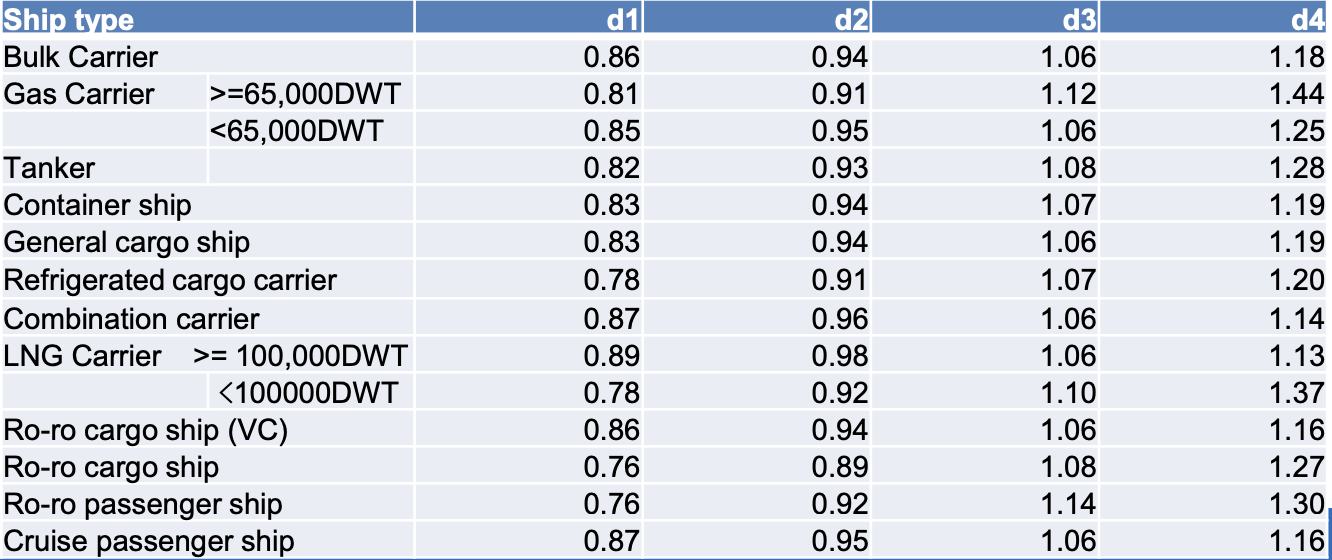
\includegraphics[width=1\textwidth]{images/dd_vecotor.png}
    \caption{$dd$ vectors for determining the rating boundaries of ship types}
    \label{dd_vecotor}
\end{figure}

\begin{figure}[h]
    \centering
    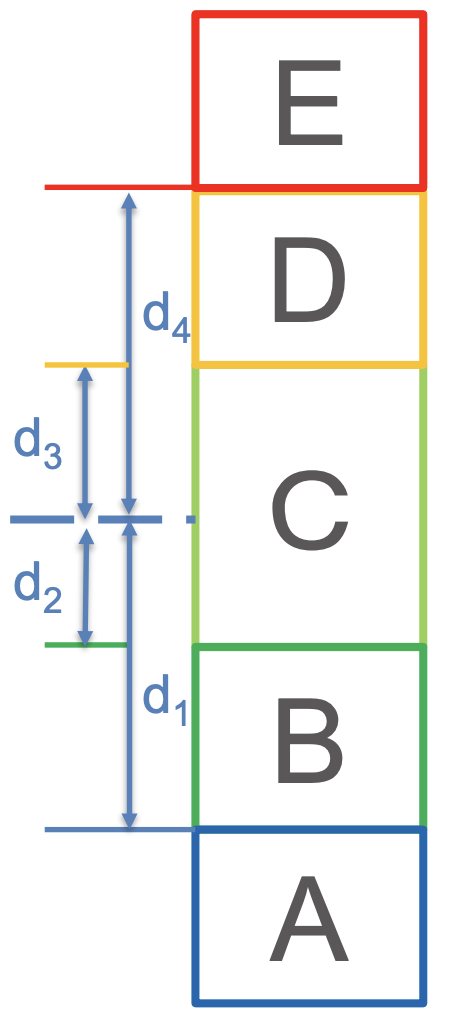
\includegraphics[width=0.2\textwidth]{images/cii_grade_dd_grade.png}
    \caption{CII grading based on $dd$ vector}
    \label{cii_grade_dd_grade}
\end{figure}

Based on figure \ref{dd_vecotor}, the CII grade can be determined as represented in figure \ref{cii_grade_dd_grade}.


Following above 6 steps, we can calculate emissions, CII, CII required, CII reference and CII grade for each vessel.
Results can be stored in a SQL table for further analysis.
For each segment, we can perform above steps as showing in Listing \ref{analysis_segment}

\begin{lstlisting}[language=python, caption=Analysis for capsize segment, label=analysis_segment]
    capsizeImoQeury = spark.sql(f"""
                       select distinct(imo) from capesize.tradeFlow as st
                       """)
    startDate = '2022-01-01'
    endDate = '2022-12-31'
    segment = 'capesize'
    capeSize = capsizeImoQeury.toPandas()
    for imo in capeSize['imo']:
    imoCIIData = getCIIGradeByImo(imo, startDate, endDate, segment, 5)
    df = pd.DataFrame([imoCIIData])
    spark.createDataFrame(df).write.mode("append").saveAsTable("emissions.capesize_cii_2022_v3")
    time.sleep(5)
\end{lstlisting}

In listing \ref{analysis_segment}, we are getting distinct IMO numbers for capsize segment.
Then for each IMO number, we are calling \texttt{getCIIGradeByImo} function to get emissions, CII, CII required, CII reference and CII grade.
Using $spark.createDataFrame(df).write()$ we are storing results in SQL table.

Based on the data obtained so far, we will analysis the results in the next chapter.



\chapter{Results and Discussion}

Based on the preceding analysis, following parameters were derived for each vessel, assuming they will engage in similar trade flows as observed in 2022, but in the year 2023. 
The vessels have been categorized into segments, facilitating a more intricate examination of the outcomes. The segments encompassed within this report include Capesize, Panamax, Supramax, Aframax, Suezmax, VLGC, and VLCC.

The analysis encompassed a total of 9,406 vessels. 
The parameters acquired for each vessel comprise an array of emissions and indices, contributing to a comprehensive assessment. 
These parameters encompass CO2 emissions, SO2 emissions, NOx emissions, PM emissions, NMVOC, CH4, N2O, CO, Black Carbon, Organic Carbon, EEOI, CII, and CII grade.

\section{Grade Distribution}

\begin{figure}[h]
    \centering
    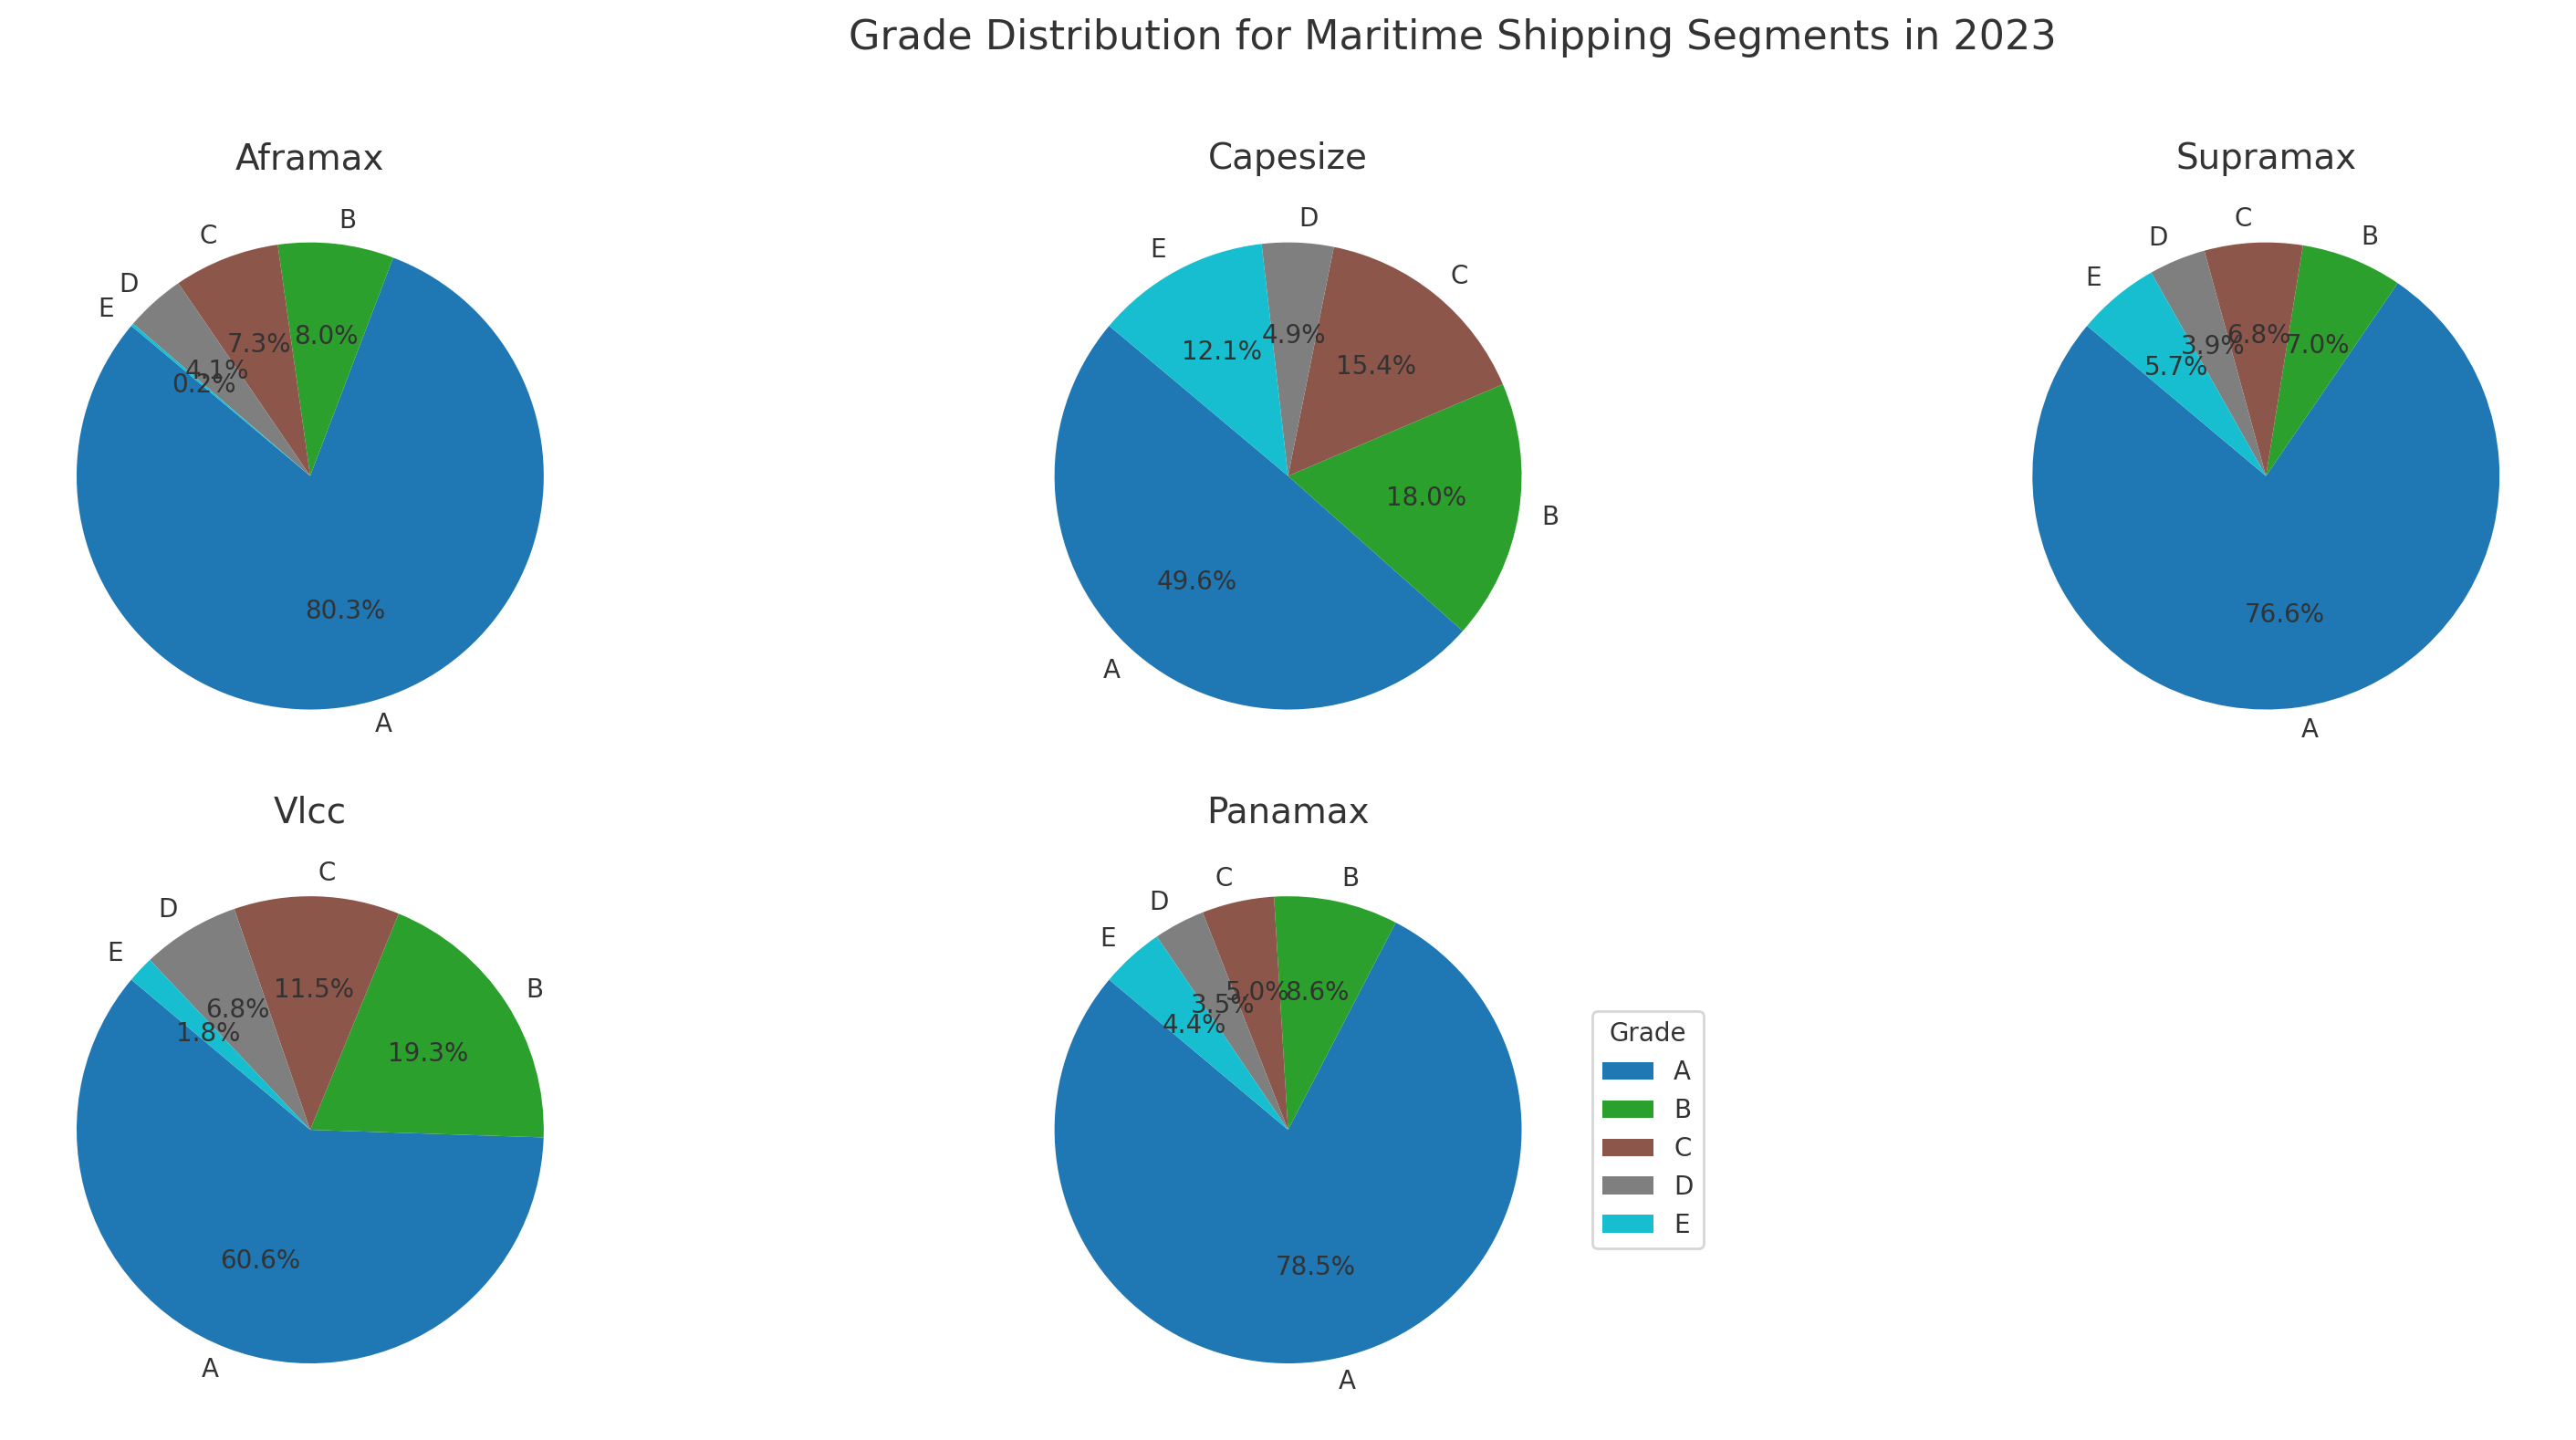
\includegraphics[width=0.8\textwidth]{images/grade_distribution.png}
    \caption{Grade Distribution}
    \label{grade_distribution}
\end{figure}


\begin{figure}[h]
    \centering
    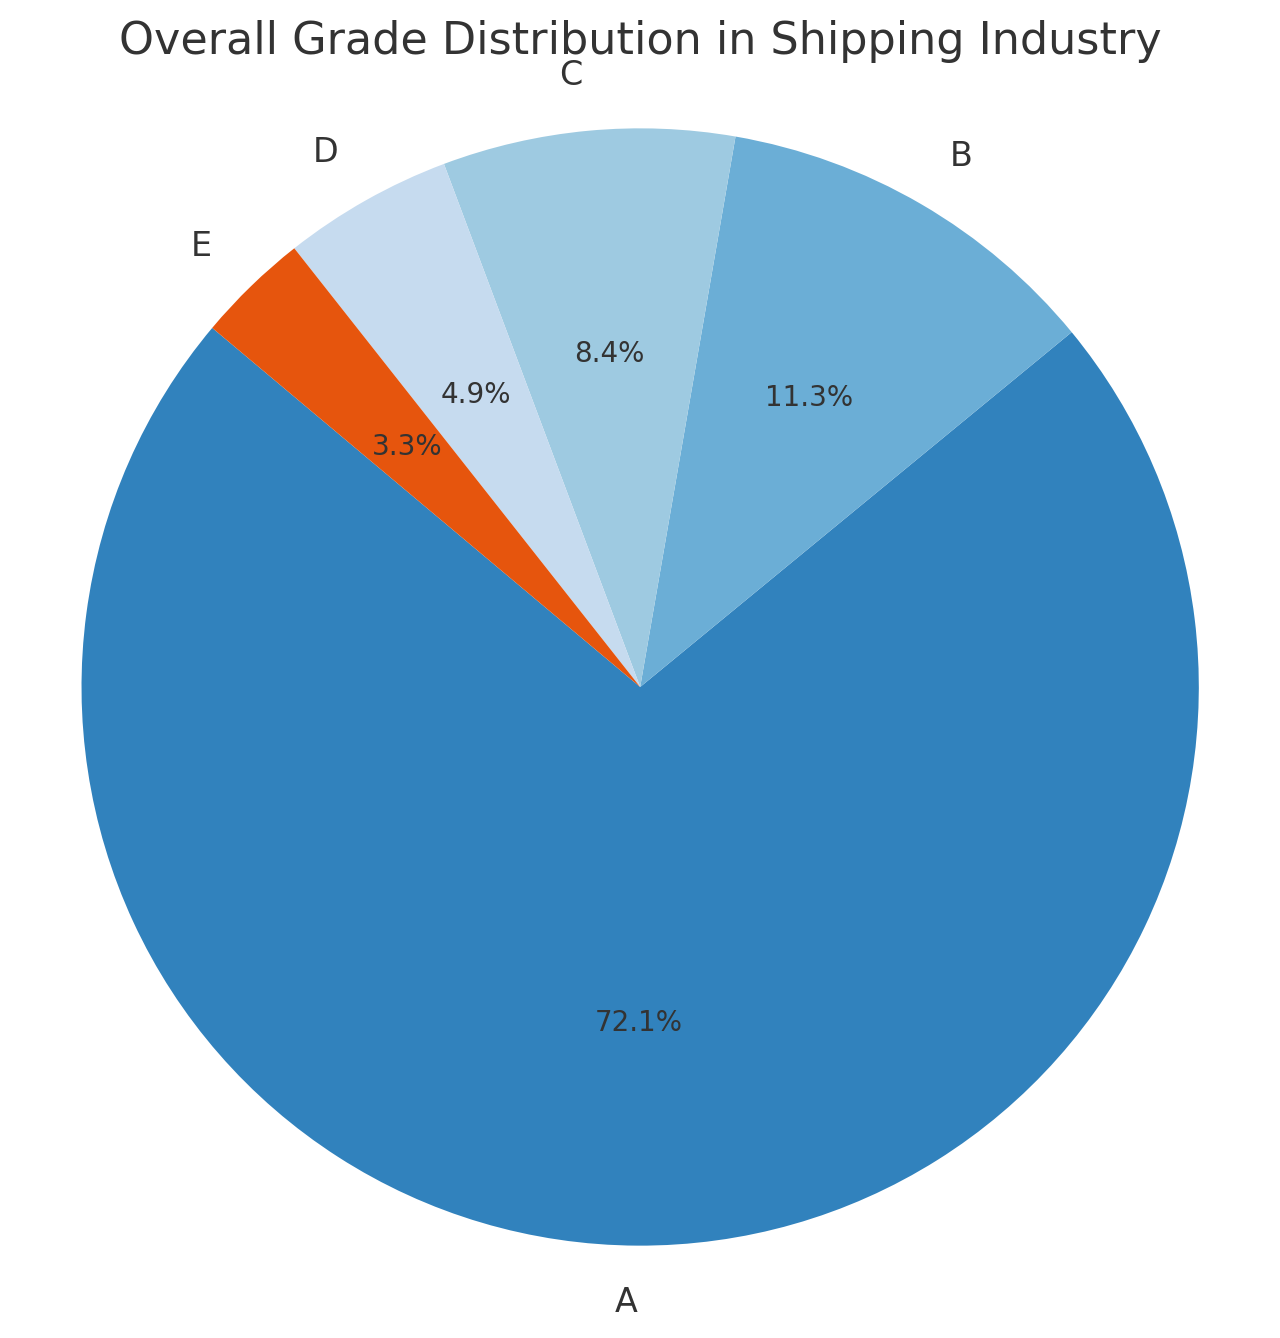
\includegraphics[width=0.8\textwidth]{images/combined_grade.png}
    \caption{Combined Grade}
    \label{combined_grade}
\end{figure}

The pie chart analysis of vessel grades across different maritime shipping segments in Figure \ref{grade_distribution}, 
along with the combined view in Figure \ref{combined_grade}, offers a nuanced understanding of the quality and compliance distribution within the industry as of 2023.


Most of segments shows similar distribution of grades, with Grade A being in between 60\% to 80\% while Grade D and E being around 10\%.
This can be reflected in combined chart too. Though capesize is an exception with only about 50\% of vessels in Grade A and alomst 16\% with grade D and E.

The combined pie chart encapsulates the overall landscape, showing 69.5\% of vessels in Grade A, and 10\% in Grade D and E.

The segment-specific insights reveal subtle variations that may be influenced by factors such as vessel size, purpose, technological capabilities, and market demands. 
Understanding these variations is essential for targeted interventions and strategies to further enhance quality and compliance.

In conclusion, the pie chart analysis paints a vivid picture of the maritime shipping industry's commitment to high standards as reflected in the grades. 
It also emphasizes the need for continuous innovation, particularly in the face of stricter grading systems in the future. 
The segment-wise insights provide valuable guidance for industry stakeholders, regulators, and policymakers, facilitating data-driven decision-making and fostering a culture of continuous improvement and adaptation.


\section{Projected Grade Trend}

\begin{figure}[h]
    \centering
    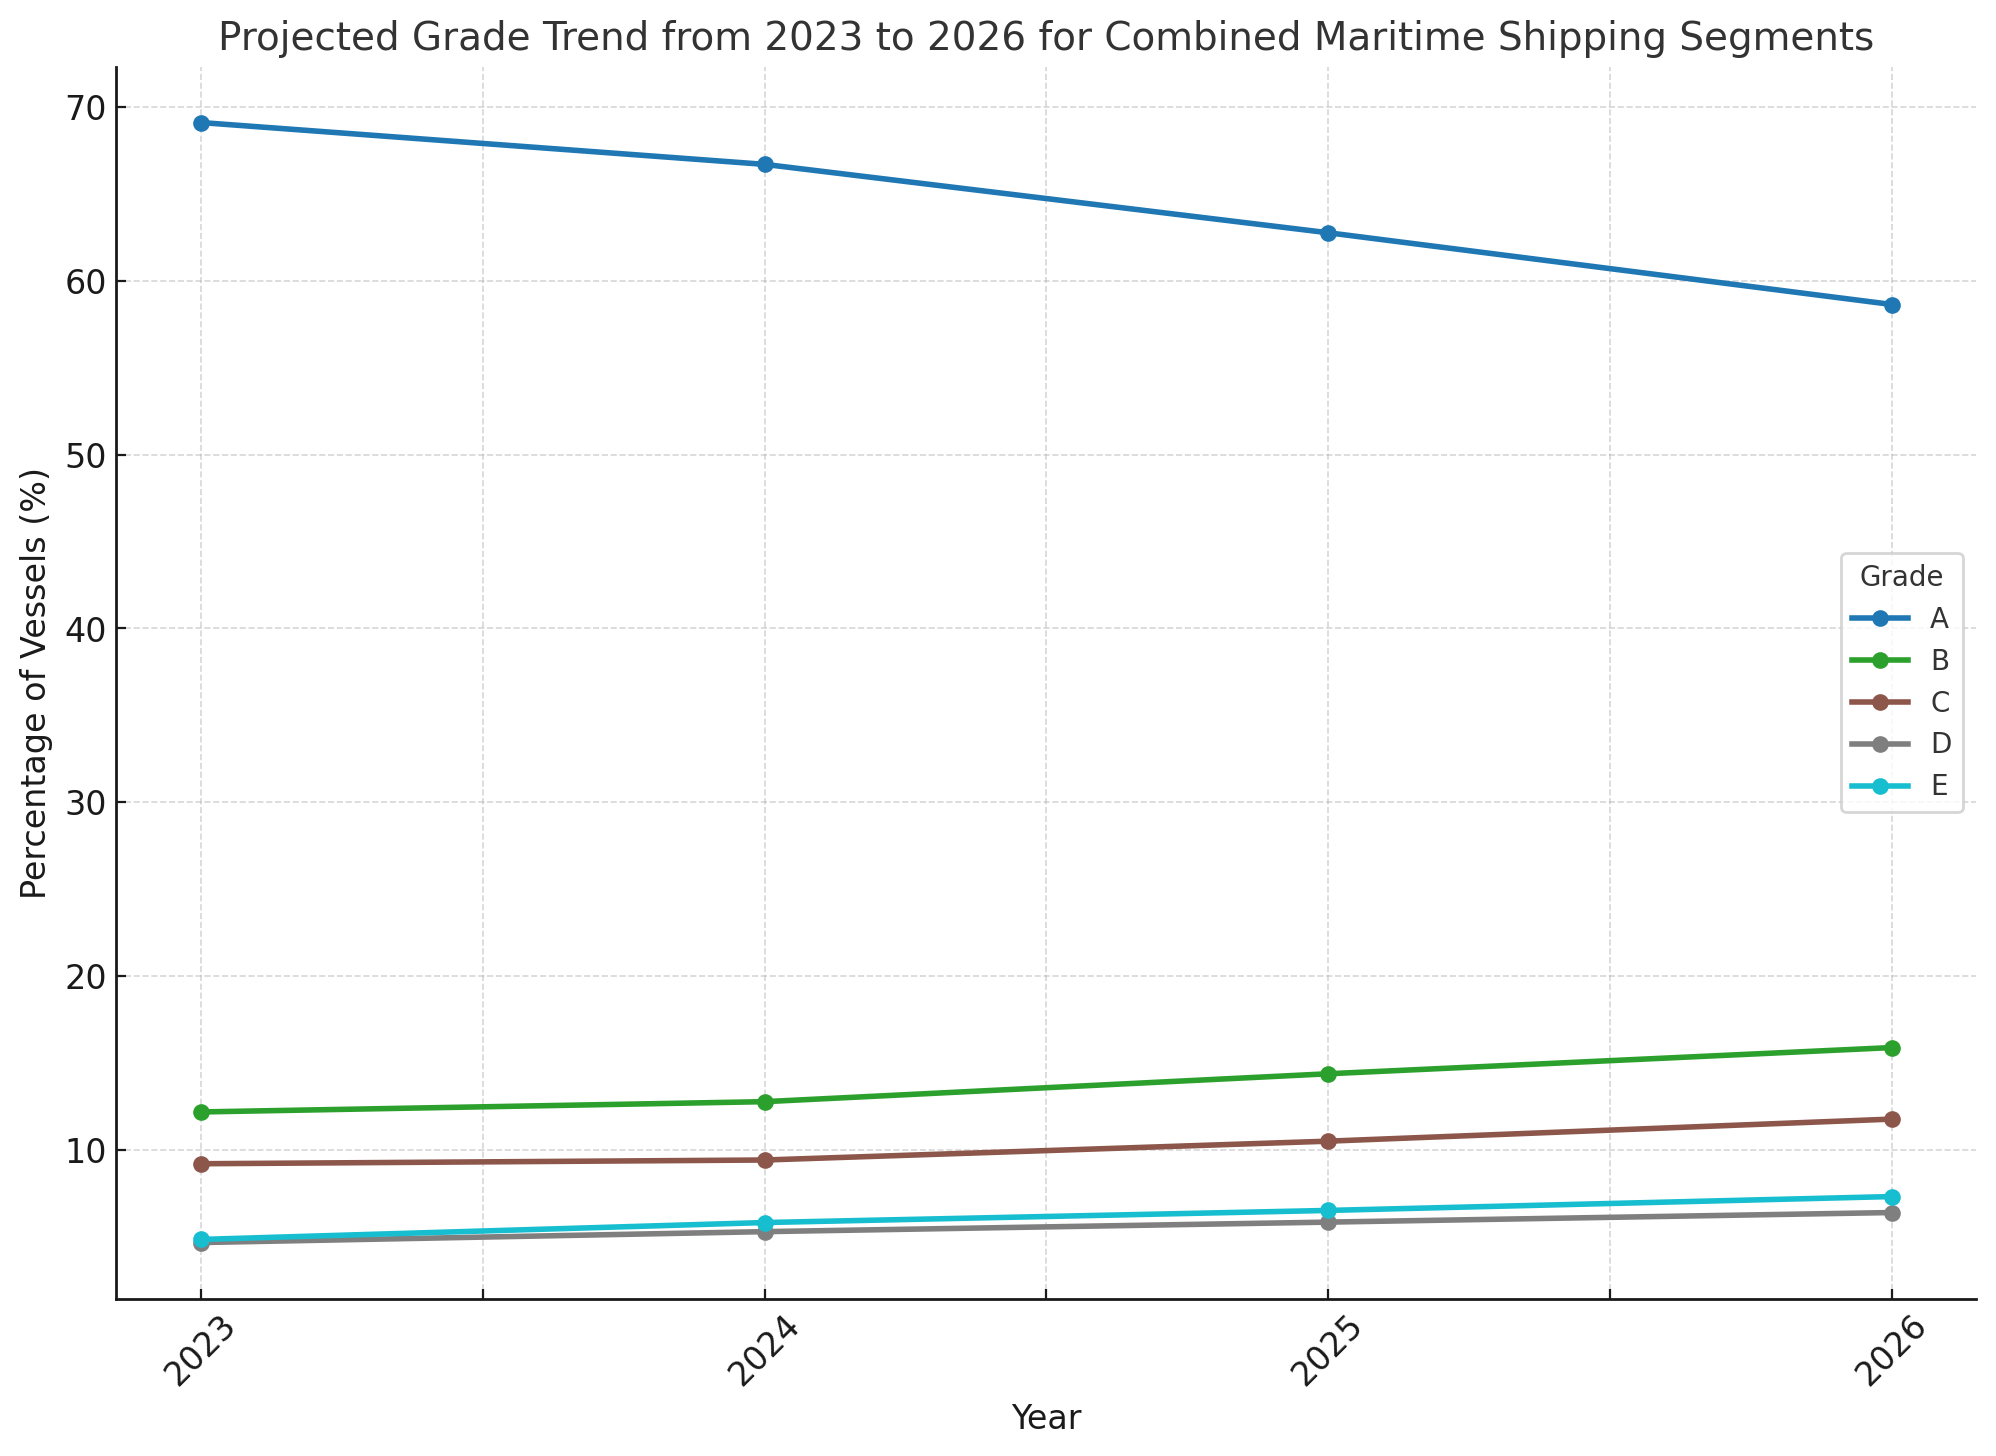
\includegraphics[width=0.8\textwidth]{images/grade_trend.png}
    \caption{Projected Grade Trend}
    \label{grade_trend}
\end{figure}

The analysis of the projected grade trend from 2023 to 2026 in plot \ref{grade_trend} unveils a compelling narrative of the industry's response to an increasingly stringent grading system. 
The most pronounced observation is the decline in the percentage of vessels achieving Grade A, falling from 69\% in 2023 to less than 60\% in 2026. 
This reduction is not indicative of a decline in quality or compliance but rather a reflection of the escalating standards and criteria set by the grading authorities.

This trend underscores the industry's challenge to keep pace with evolving regulations and the imperative for continuous innovation and improvement. 
As the grading system becomes more demanding, the criteria for achieving Grade A are elevated, pushing some vessels into the B and C categories. 
The growth in Grades B and C, from about 12.18\% to 16\% and 9\% to 12\% respectively, illustrates this shift.

Even the slight increases in Grades D and E, though representing a smaller fraction of the fleet, emphasize the pressing need for maritime shipping to adapt, innovate, and invest in new technologies and practices. 
The trend towards more rigorous grading is likely driven by global efforts to enhance environmental sustainability, safety standards, and overall efficiency within the maritime sector.

The observed grade trend serves as both a challenge and an opportunity for maritime shipping. 
It calls for a proactive and strategic approach, where shipping companies must embrace research and development, adopt advanced technologies, and foster a culture of excellence. 
The industry must recognize that the path to high grades is dynamic and requires ongoing commitment to align with the progressive standards.

In conclusion, the projected grade trend from 2023 to 2026 is a testament to the maritime shipping industry's evolving landscape. 
It emphasizes the critical role of innovation in meeting the future demands of a stricter grading system. 
This trend offers valuable insights for policymakers, regulators, and industry leaders, guiding them towards collaborative efforts that ensure the maritime shipping industry not only maintains its current standards but continually strives to reach new heights of quality and responsibility.

\section{EEOI vs Grade}

\begin{figure}[h]
    \centering
    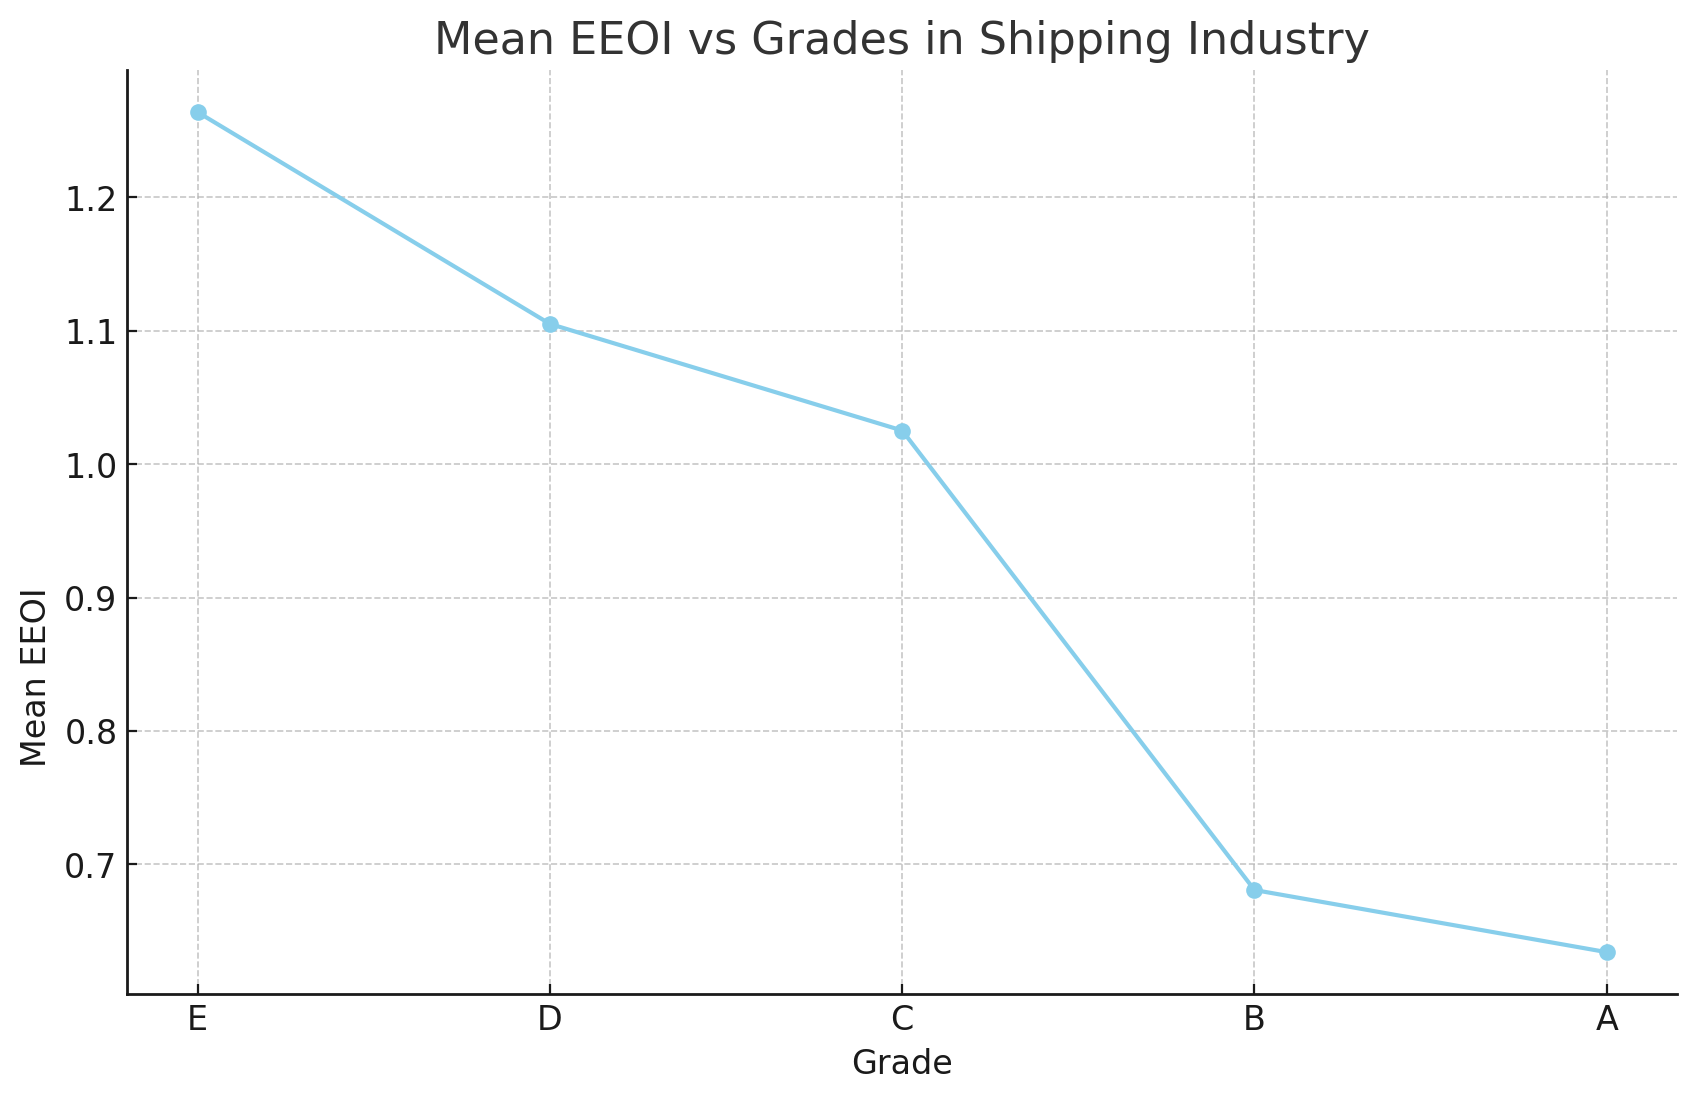
\includegraphics[width=0.8\textwidth]{images/eeoi_grade.png}
    \caption{Mean EEOI vs Grade}
    \label{eeoi_grade}
\end{figure}

The above Figure \ref{eeoi_grade} represents relationship between EEOI and grade.

Lower Efficiency Operational Indicator (EEOI) means vessels uses less fuel to achieve same amount of work.
The relationship between the Energy EEOI and vessel grades in the maritime shipping industry offers a logical and meaningful correlation. 
Lower EEOI values, signifying better energy efficiency, correspond to higher vessel grades (A being the highest). 
The grading system incentivize energy-efficient practices and provides a transparent metric for evaluating vessel quality and environmental responsibility.

\section{Average speed vs Grade}
\begin{figure}[h]
    \centering
    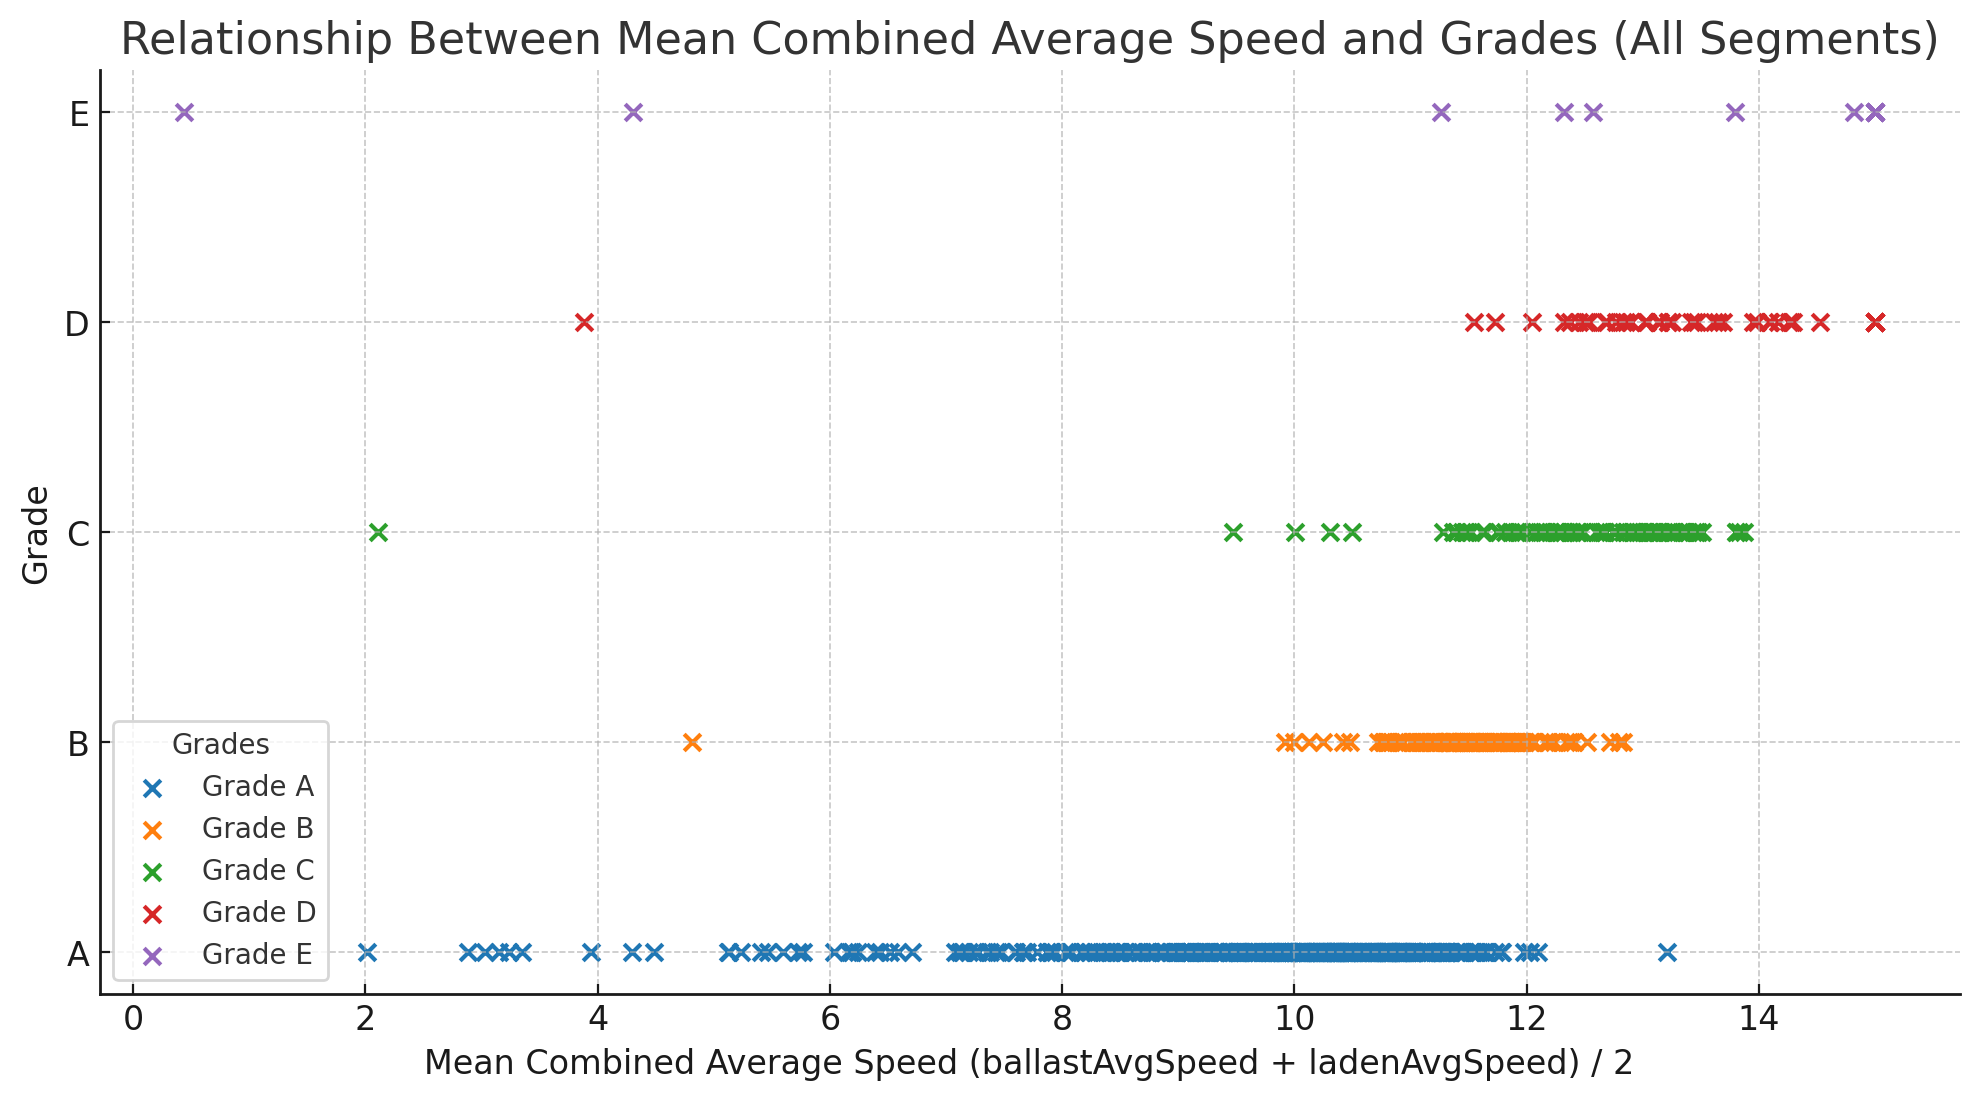
\includegraphics[width=0.8\textwidth]{images/grade_speed.png}
    \caption{Average Speed vs Grade}
    \label{grade_speed}
\end{figure}

To understand if speed has any impact on grade, scatter plot of average speed vs grade is plotted.
From the plot \ref{grade_speed} it is noticed that vessels with lower speed have better grade. 
It is very clear that almost all the vessels with speed 12.5 knots or more have grade C or below.

\section{Grade by Build Country}

\begin{figure}[h]
    \centering
    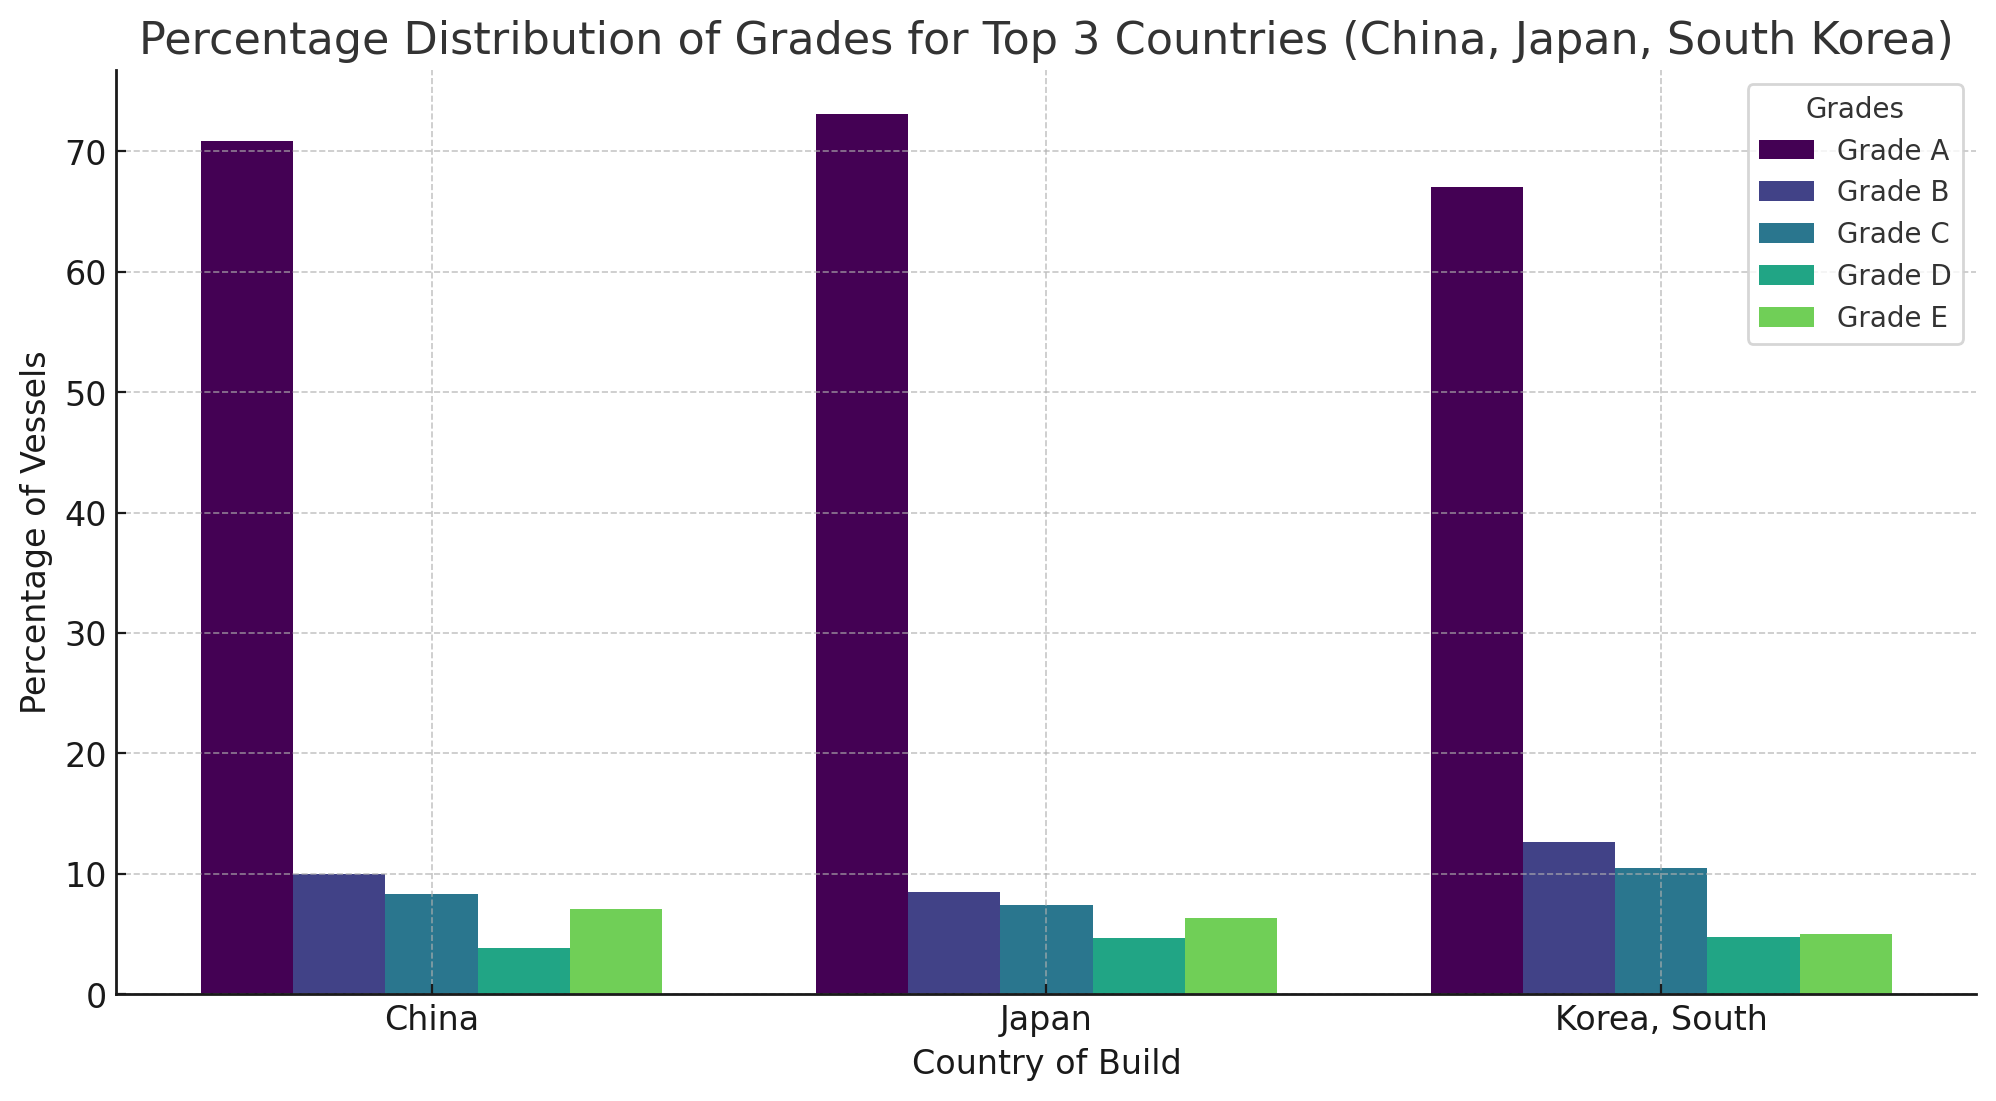
\includegraphics[width=0.8\textwidth]{images/grade_by_build_country.png}
    \caption{Grade By Build Country}
    \label{grade_by_build_country}
\end{figure}

Country where vessels are built can effect grade significantly as many parameters like materials, technology, regulations etc. can vary from country to country.
To verify this hypothesis, grade distribution by build country is plotted in Figure \ref{grade_by_build_country}.
To make the plot more readable, only top 3 countries China, Japan and South Korea were considered.

From plot \ref{grade_by_build_country} it is clear that vessels built in Japan have better grade than vessels built in China or South Korea.

\section{Addressing Low Rating}

When a ship's Carbon Intensity Indicator (CII) receives a low grade of D for three consecutive years or E for one year, specific measures must be undertaken to address and improve the situation. 
As per the regulations, a corrective action plan must be submitted and approved. 

Some of the strategies include the use of alternative fuels, which may require significant investment but have high effectiveness; 
the application of low friction paint and Energy Saving Devices (ESD) to improve hardware; 
voyage optimization and fleet optimization, which may require preliminary examination but have a low to middle cost and depend on the ship's specific situation; 
and slow steaming, which requires an analysis of monitoring results and estimation of cost-effectiveness. 
These methods indicate a multifaceted approach that considers cost, effectiveness, and specific ship characteristics to overcome the challenges associated with a low CII rating. 
The strategies emphasize both technological improvements and operational adjustments, reflecting an integrated approach to enhance environmental performance.


\section{Emissions}

Based on AF code emission API and vessel parameters, various emissions are calculated for each vessel grouped by segment.

\begin{figure}[h]
    \centering
    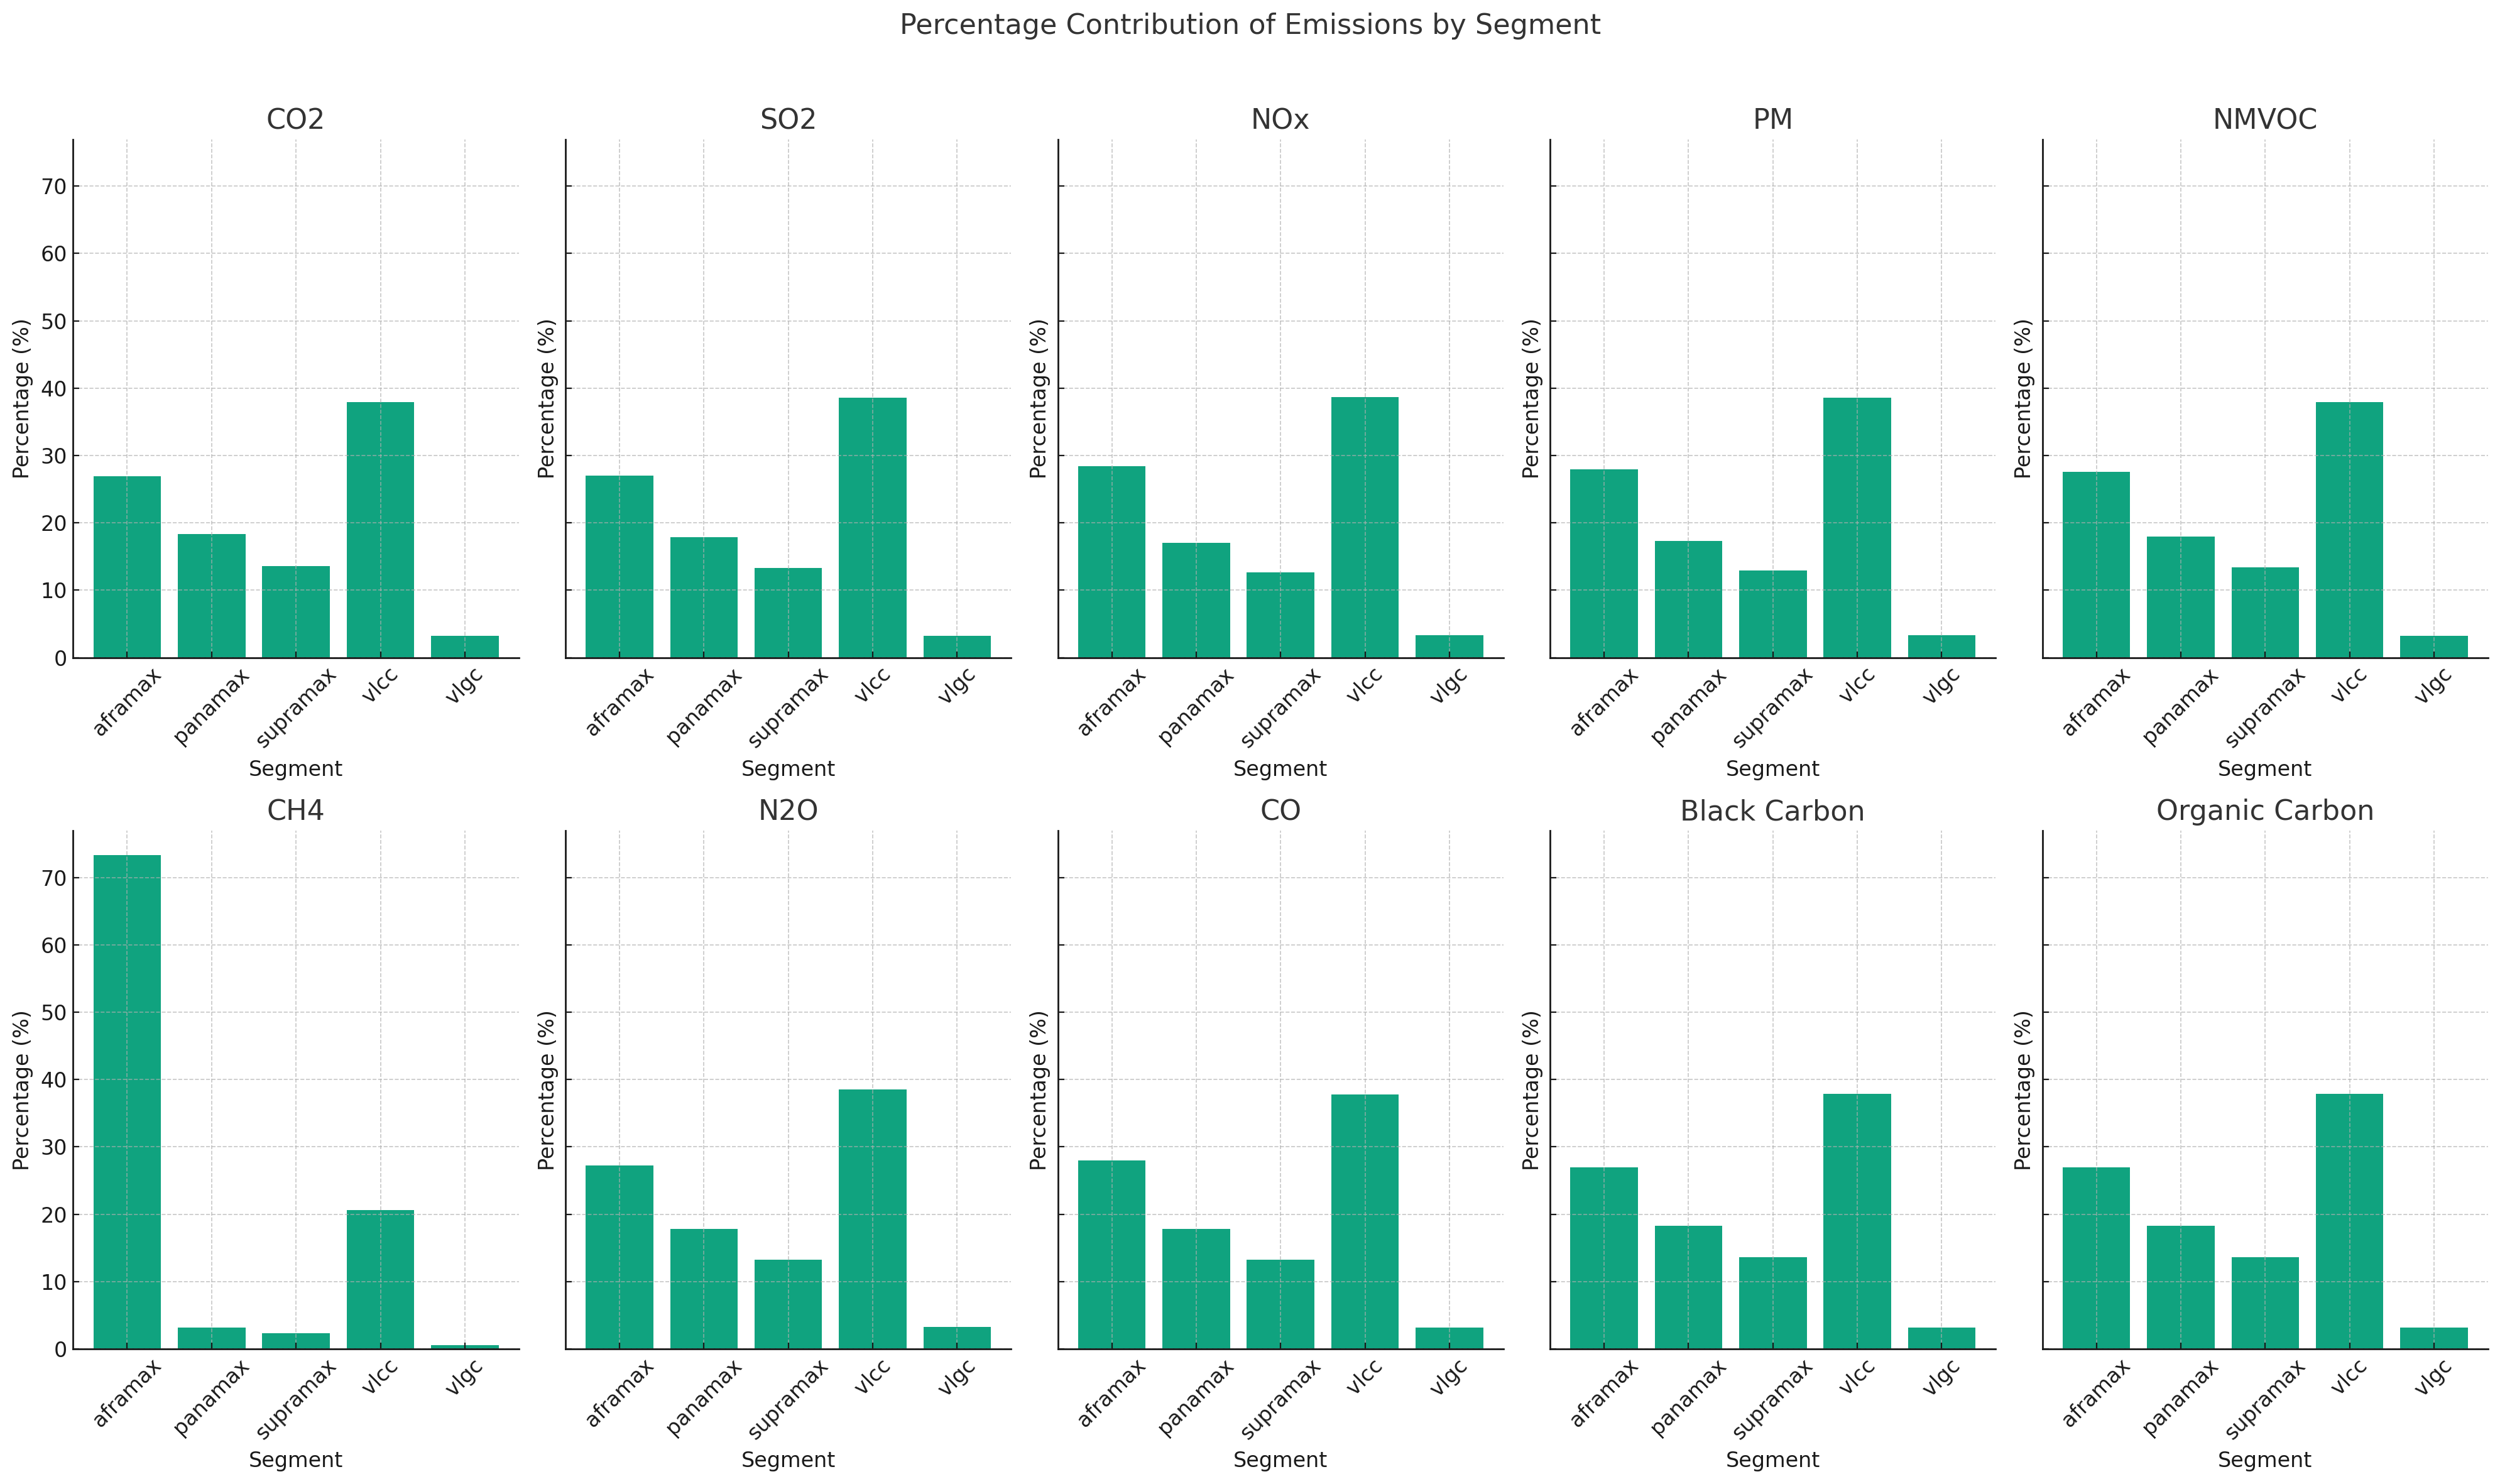
\includegraphics[width=0.8\textwidth]{images/segment_emissions.png}
    \caption{Percentage of Emissions by Segment}
    \label{segment_emissions}
\end{figure}

Figure \ref{segment_emissions} shows percentage of emissions by segment.
The analysis reveals a diverse emission profile across segments such as VLCC, VLG, Aframax, Panamax, Capesize, and Supramax. 
Notably, the VLCC segment emerges as a significant contributor to emissions such as CO2, SO2, and NOx, highlighting potential areas for emission reduction strategies.

\chapter{Conclusion}

Initially, dividing the vessels into segments and assigning Grade from A to E for given year as Carbon intensity indicator provides a clear picture of the carbon emissions of the vessel.
Through the analysis of more than 9000 vessels, it was found that the average grade of vessels has been decreasing over the years. 
This shows that the carbon emissions of vessels has been increasing over the years.
If the emissions during the voyage is not reduced, Carbon intensity indicator of more and more vessels will fall under D or E grade. 

The thesis also shows that one of the key factor effecting the carbon emissions is the speed and EEOI of the vessel.
Using alternative fuels, applying low friction paint, voyage route optimization, and using latest hardware are some of the practical solutions to reduce the carbon emissions of the vessels


This study delved into a comprehensive investigation of carbon emissions in maritime shipping, a crucial yet intricate facet of the industry. Through the course of this research, several key questions were addressed:

\begin{enumerate}
    \item \textbf{Understanding Complexity with Simplicity}: The analysis demonstrated that even the multifaceted nature of emissions could be understood through a well-structured and comprehensible system. By breaking down complex elements, the thesis facilitated a clearer grasp of emissions dynamics.
    \item \textbf{Categorization of Vessels}: The categorization of vessels into distinct segments such as Capesize, Panamax, Supramax, and others enabled a more nuanced examination of carbon emissions. This segmentation provided unique insights into each category's characteristics and emissions behavior.
    \item \textbf{Factors Affecting Carbon Emissions}: A comprehensive analysis was conducted to identify the multitude of factors affecting a vessel's carbon emissions. This understanding forms a foundation for more targeted and effective emissions control strategies.
    \item \textbf{Realistic Emissions Reduction}: The thesis explored various cost-effective and practical measures to reduce carbon emissions. These findings not only contribute to environmental sustainability but also offer realistic paths for industry implementation.
\end{enumerate}

This thesis set the stage for future research that continues to push the boundaries of our understanding and capabilities. 
Looking ahead, there are several promising avenues for future research. 
The consideration of port emissions alongside voyage emissions presents an opportunity for a more holistic view of maritime carbon footprints. 
Additionally, analyzing more vessel segments will further refine our understanding and provide more detailed insights. 
These future efforts align with the ongoing pursuit of environmental responsibility and efficiency in the maritime shipping industry.

In conclusion, this thesis has made a significant contribution to the field by unraveling the complexities of maritime shipping's carbon emissions. 
It has provided valuable insights, practical solutions, and set the stage for future research that continues to push the boundaries of our understanding and capabilities.



\addcontentsline{toc}{chapter}{Bibliography}
\printbibliography

\end{document}